\documentclass[letterpaper, 12pt, oneside]{tesis}
\graphicspath{{figuras/}}

\usepackage[spanish]{babel}
%\usepackage[spanish]{hyphenat}
\usepackage{hyphenat}

\usepackage[square, numbers, comma, sort&compress]{natbib}
\usepackage{verbatim}
\usepackage{tikz}
\usepackage{fancyvrb}
\usepackage{enumerate}
\usepackage{paquetes/vector}
\usepackage{color}
\usepackage{hyperref}
\usepackage{amsthm}
\usepackage{amsfonts}
\usepackage{algorithmic}
\usepackage{algorithm}
\usepackage{float}
\usepackage{epigraph}
\usepackage{array}
\usepackage{tabularx}
\usepackage{caption}
\usepackage[utf8]{inputenc}
\usepackage[fixlanguage]{babelbib}
%\usepackage[letterpaper, inner=3cm, outer=2cm]{geometry}
%\addtolength[\topmargin]{-1.5cm}
%\addtolength[\textheight]{4cm}

%\usepackage{setspace,cite} % Doble espacio para texto, espacio singular para
                           % los caption y pie de pagina

\hypersetup{urlcolor=blue, colorlinks=false}
\numberwithin{algorithm}{chapter}

\newcommand{\ALG}{Lista de Algoritmos}
\renewcommand*\listalgorithmname{\ALG}
\renewcommand{\tablename}{Tabla}
\renewcommand{\spanishtablename}{Tabla}
\renewcommand*\listtablename{Lista de Tablas}
\newcommand\listsymbolname{Acrónimos}
\newcommand{\tup}[1]{\langle #1 \rangle}
\floatname{algorithm}{Algoritmo}
\newcommand{\A}{\ensuremath{\mathcal{A}}}
\newcommand{\LPO}{\text{LPO}}
\newcommand{\LSO}{\text{LSO}}
\newcommand{\SO}{\ensuremath{\text{SO}}}
\newcommand{\SOE}{\ensuremath{\text{SO}\exists}}
\newcommand{\SOA}{\ensuremath{\text{SO}\forall}}
\newcommand{\SOEA}{\ensuremath{\text{SO}\exists\forall}}
\newcommand{\SOAEA}{\ensuremath{\text{SO}\forall\exists\forall}}
\newcommand{\Q}{\ensuremath{\mathcal{Q}}}
\newcommand{\struc}{\text{STRUC}}
\newcommand{\FT}{\ensuremath{\mathfrak{F}}}
\newcommand{\eq}{\equiv}
\newcommand{\pwin}{mkspw}
\renewcommand{\models}{\vDash}

\parindent 3ex % Agrega sangrías de 3 espacios (3 veces el espacio de la x)
\setlength{\baselineskip}{1.5pt} % Interlineado 1.5
\setlength{\parskip}{16.5pt} % Interparrafo 16.5pt
%\oddsidemargin 3cm
\topmargin 2cm

%! referencias manera estandar

%%%% Título
\begin{titlepage}
	\title{\vspace{-2cm} 
\includegraphics[width=1.2in]{./usb.png} \\[.2cm]
		\large Universidad Simón Bolívar \\
		Decanato de Estudios Profesionales \\
		Coordinación de Ingeniería de la Computación
		\vfill
		\LARGE Reducciones automáticas de problemas de decisión en problemas de
        planificación \vfill}
	\author{Por: \\
		Aldo Fabrizio Porco Rametta \\
		Alejandro Machado González \\[1.2cm]
		Realizado con la asesoría de: \\
		Prof. Blai Bonet\\[1.2cm]
		PROYECTO DE GRADO \\
Presentado ante la Ilustre Universidad Simón Bolívar \\
como requisito parcial para optar al título de \\
Ingeniero de Computación}
    \date{Sartenejas, Diciembre de 2012}
\end{titlepage}
%%%% Título

\begin{document}

\frontmatter

\maketitle
\setstretch{1.3}

%% Define the page headers using the FancyHdr package and set up for one-sided printing
%\fancyhead{}  % Clears all page headers and footers
%\rhead{\thepage}  % Sets the right side header to show the page number
%\lhead{}  % Clears the left side page header
%
%\pagestyle{fancy}  % Finally, use the "fancy" page style to implement the FancyHdr headers
%
%%% ----------------------------------------------------------------
%% The "Funny Quote Page"
%\setcounter{page}{2}
%\pagestyle{empty}  % No headers or footers for the following pages
%
%\null\vfill
%% Now comes the "Funny Quote", written in italics
%\textit{``El hombre razonable se adapta al mundo; el irrazonable intenta adaptar
%el mundo a si mismo. Así pues, el progreso depende del hombre irrazonable.''}
%
%\begin{flushright}
%George Bernard Shaw
%\end{flushright}
%
%\vfill\vfill\vfill\vfill\vfill\vfill\null
%\clearpage  % Funny Quote page ended, start a new page
%%% ----------------------------------------------------------------
%
%%% ----------------------------------------------------------------

%The Abstract Page

\addtotoc{Resumen}  % Add the "Abstract" page entry to the Contents
\abstract{
\addtocontents{toc}{\vspace{1em}}  % Add a gap in the Contents, for aesthetics
Aquí va el resumen.

\noindent \textbf{Palabras clave}: Planificación Automática, Teoría de
Complejidad, Inteligencia Artificial.

\clearpage % Abstract ended, start a new page
%% ----------------------------------------------------------------

\setstretch{1.3}  % Reset the line-spacing to 1.3 for body text (if it has changed)

% The Acknowledgements page, for thanking everyone
\acknowledgements{
\addtocontents{toc}{\vspace{1em}}  % Add a gap in the Contents, for aesthetics
Agradecimientos aquí.
}

\clearpage  % End of the Acknowledgements

\pagestyle{fancy}  %The page style headers have been "empty" all this time, now use the "fancy" headers as defined before to bring them back


%% ----------------------------------------------------------------
\lhead{\emph{Índice General}}  % Set the left side page header to "Contents"
\tableofcontents  % Write out the Table of Contents

%% ----------------------------------------------------------------
\lhead{\emph{Índice de Figuras}}  % Set the left side page header to "List if figuras" 
\listoffigures  % Write out the List of figuras

%% ----------------------------------------------------------------
\lhead{\emph{Índice de Tablas}}  % Set the left side page header to "List of Tables"
\renewcommand*\listtablename{Lista de Tablas}
\listoftables  % Write out the List of Tables

%% ----------------------------------------------------------------
%\lhead{\emph{Lista de Algoritmos}} % Set the left side page header to "List of Algorithms"
%\addtotoc{Lista de Algoritmos}
%\listofalgorithms % Write out the List of Algorithms

%% ----------------------------------------------------------------
\setstretch{1.5}  % Set the line spacing to 1.5, this makes the following tables easier to read
\clearpage  % Start a new page
\lhead{\emph{Acrónimos y símbolos}}  % Set the left side page header to "Abbreviations"
\listofsymbols{ll}  % Include a list of Abbreviations (a table of two columns)
{
% \textbf{Acronym} & \textbf{W}hat (it) \textbf{S}tands \textbf{F}or \\
\textbf{LPO} & \textbf{L}ógica de \textbf{P}rimer \textbf{O}rden\\
\textbf{LSO} & \textbf{L}ógica de \textbf{S}egundo \textbf{O}rden\\
\textbf{LSO} & \textbf{T}eoría de \textbf{C}omplejidad \textbf{D}escriptiva\\
\textbf{NP} & \textbf{N}ondeterministic \textbf{P}olynomial time (clase de complejidad)\\
\textbf{PDDL} & \textbf{P}lanning \textbf{D}omain \textbf{D}efinition \textbf{L}anguage \\
\textbf{PH} & \textbf{P}olynomial \textbf{H}ierarchy (clase de complejidad)\\
\textbf{SAT} & boolean \textbf{SAT}isfiability\\
\textbf{TCD} & \textbf{T}eoría de \textbf{C}omplejidad \textbf{D}escriptiva\\
\textbf{Fun} & función total\\
\textbf{Inj} & función total inyectiva\\
\textbf{PFun} & función parcial\\
\textbf{PInj} & función parcial inyectiva\\
&\\
\hline
&\\
$\iff$ & doble implicación, si y sólo si\\
$\Rightarrow$ & implicación lógica
}

%% ----------------------------------------------------------------
% End of the pre-able, contents and lists of things
% Begin the Dedication page

\setstretch{1.3}  % Return the line spacing back to 1.3

\pagestyle{empty}  % Page style needs to be empty for this page
%\dedicatory{Dedicated to adventures...\ldots}

\addtocontents{toc}{\vspace{2em}}  % Add a gap in the Contents, for aesthetics


%% ----------------------------------------------------------------
\mainmatter	  % Begin normal, numeric (1,2,3...) page numbering
\pagestyle{fancy}  % Return the page headers back to the "fancy" style

% Include the chapters of the thesis, as separate files
% Just uncomment the lines as you write the chapters

% Chapter 1

\chapter*{Introducción} % Write in your own chapter title
\label{Intro}
\lhead{\emph{Introducción}} % Write in your own chapter title to set the page header
\addcontentsline{toc}{chapter}{Introducción}
% Descripción general
En Ciencias de la Computación se entiende por \textbf{problemas de decisión}
los problemas en los que se plantea una pregunta en un sistema formal sobre una entrada
arbitraria, cuya respuesta puede ser afirmativa o negativa.
Los problemas de decisión son interesantes porque permiten modelar y razonar
sobre aplicaciones reales. Por ejemplo, el problema de decisión de
$k$-colorabilidad pregunta si los vértices de un grafo pueden ser coloreados
con $k$ colores distintos, de modo de que a ningún par de vértices conectados
por una arista se les asigne el mismo color . En un compilador, la tarea de
asignar los valores frecuentemente utilizados a registros para
mejorar la eficiencia del código generado puede modelarse con un problema de
$k$-colorabilidad: los vértices del grafo son las variables, y si dos variables
se necesitan al mismo tiempo se coloca un arco entre ellas. Al encontrar una
forma de colorear este grafo con $k$ colores se ha hallado una forma de
utilizar $k$ registros distintos para almacenar las variables.

Los problemas de decisión pueden agruparse en distintas clases según su
complejidad. Una importante clase de complejidad es NP (siglas de
\textit{Nondeterministic Polynomial time}), a la cual pertenecen problemas
interesantes como $k$-colorabilidad, satisfacibilidad proposicional
(\textbf{SAT}) y hallar un camino \textit{hamiltoniano} en un grafo. Otra clase
más general de problemas de interés para este trabajo es PH (\textit{Polynomial Hierarchy}),
que incluye problemas computacionalmente más complejos como formas restringidas de
\textit{Quantified Boolean Formula} (QBF).

El área de investigación de planificación automática estudia una forma general
de resolución de problemas utilizando \textbf{planes}. Un problema de planificación
consiste de un estado inicial, un conjunto de estados finales y un conjunto de
acciones posibles. Luego, la tarea del \textbf{planificador} 
consiste en encontrar una secuencia de acciones que conduzca
el estado inicial hasta un estado final, o determinar que tal secuencia de
acciones no existe.

Este trabajo se enfoca en el desarrollo de una herramienta que permite
traducir o, en lenguaje más formal, \textbf{reducir} un problema de
decisión perteneciente a las clases NP o PH codificado en lógica de segundo orden,
a un problema de planificación automática. 
La motivación para realizar esta herramienta es que
existen planificadores muy eficientes, pero no es trivial
expresar un problema de decisión cualquiera en términos de estado inicial,
estados finales y acciones, como lo requieren los
planificadores. A veces, la utilización de un lenguaje declarativo es una forma
más concreta y directa para la descripción de un problema de decisión en
particular. En estos casos, es preferible modelarlo en un lenguaje de más alto
nivel y que la herramienta lo reduzca a un formato de entrada aceptado por
los planificadores, los cuales pueden proceder entonces a computar su solución.

% Trabajos anteriores
Otros autores ya han utilizado fragmentos de la lógica de segundo orden como un lenguaje de
programación declarativo. En la obra de \cite{reiter:cwa} se describe un
lenguaje de reglas y consultas a bases de datos que es un subconjunto de
PROLOG, llamado DATALOG. A su vez, \cite{cadoli:npspec} presentan una
extensión de este lenguaje que permite la codificación de problemas NP y
se desarrolla un método para compilar los problemas a código de PROLOG, el cual
fue probado con pequeñas instancias del \textbf{problema de la mochila}
(\textit{knapsack problem}) y el \textbf{problema del viajante}
(\textit{traveling salesman problem}).

\cite{mitchell:npsearch} proponen, por su parte, el lenguaje de
Extensión de Modelos (MX), que es conceptualmente muy cercano a la lógica de
segundo orden. Este trabajo se enfoca en la descripción formal del lenguaje y
en discutir la posibilidad de diseñar un solucionador. En esta sección, los
autores aconsejan la realización de una traducción a otro lenguaje para el cual
existan solucionadores: es precisamente esto lo que se ha hecho en el presente
trabajo con la función que traduce descripciones declarativas a problemas
de planificación, área para la cual existe una amplia variedad de solucionadores.

Otro trabajo relacionado a este proyecto es el de \cite{cadoli:safedelay}. Los
autores presentan una manera de razonar sobre los problemas de
decisión, intentando reformularlos para hacerlos más fáciles de resolver. Se
utilizan sistemas especializados para la modelación de restricciones y
solucionadores provenientes de muchos sub-campos de la Inteligencia Artificial.
Sin embargo, dependiendo del solucionador, se podría requerir que la fórmula
declarativa a solucionar esté en un formato particular, lo cual no es tan
conveniente como el enfoque ``independiente del dominio'' que provee la
planificación automática.

El objetivo general del proyecto es permitir la resolución de problemas
NP y de la jerarquía polinomial (PH) expresados a través de un lenguaje declarativo basado en 
la lógica de segundo orden.
Al alcanzar este objetivo, problemas cuya aplicación es
ampliamente conocida en Ciencias de la Computación podrán ser expresados
en un lenguaje conciso y ser resueltos sin la intervención del usuario luego de
la fase de modelación.

A fin de lograr el objetivo general, se plantean las siguientes metas
específicas:
\begin{itemize}
\item El desarrollo de una herramienta que procese la descripción lógica de un problema 
en NP o PH y genere automáticamente un problema de planificación equivalente 
formulado en el lenguaje PDDL (\textit{Planning Domain Definition Language}),
de uso estándar en la comunidad de planificación automática.
\item Una interfaz \textit{web} para este sistema que permita un acceso flexible
y rápido al traductor.
\end{itemize}

% Organización
Este trabajo está dividido en cinco capítulos. El primer capítulo aporta las
bases teórica sobre la que está fundamentada la traducción, incluyendo una
introducción a las áreas de planificación automática y complejidad descriptiva.
En el segundo capítulo se describe el lenguaje lógico diseñado para la
formulación de problemas a alto nivel, se presenta una reducción base del
fragmento de la lógica de segundo orden que captura a la clase NP
al lenguaje PDDL y se demuestran las propiedades formales de esta
traducción. 
%En el capítulo 3 se discuten algunas optimizaciones aplicadas sobre
%la función de reducción que permiten la generación de problemas de
%planificación menos complejos sin alterar las propiedades formales básicas de
%la traducción a NP. 
El capítulo 3 presenta una extensión de la herramienta que
permite traducir problemas más generales, pertenecientes a la jerarquía
polinomial.
El capítulo 4 trata sobre cómo fueron diseñados y llevados a
cabo experimentos sobre diferentes problemas en NP y PH traducidos con la herramienta,
además de ofrecer una discusión de los resultados obtenidos. Finalmente, el
capítulo 5 contiene conclusiones, recomendaciones e ideas para trabajos
futuros.

Parte de este trabajo ha sido publicado en la \textit{21st International Conference on
Automated Planning and Scheduling} (ICAPS 2011;
\citeauthor{porco:npreductions}), y
enviado como artículo de investigación a la \textit{23rd International
Conference on Automated Planning and Scheduling} (ICAPS 2013).

%2. ACTIVIDADES QUE INVOLUCRA EL PROYECTO: 
%a. Investigación sobre el material teórico que permiten relacionar la teoría de complejidad computacional con complejidad descriptiva (lógica)
%b. Especificación del lenguaje lógico propuesto para realizar formulaciones, gramática y semántica de las construcciones
%c. Definición de la traducción del lenguaje lógico a PDDL, demostración de la correctitud y completitud de esta equivalencia
%d. Desarrollo del analizador léxico y sintáctico que permita reconocer este lenguaje
%e. Implementación de algoritmos para el post-procesamiento del árbol sintáctico para la simplificación de la fórmula lógica a formas canónicas
%f. Implementación de la traducción definida anteriormente sobre el árbol sintáctico de la fórmula procesada
%g. Evaluación experimental del desempeño de planificadores (del estado del arte) sobre fórmulas que corresponden a varios dominios
%h. Programación de una herramienta integral web que sirva como una interfaz ante el usuario para acceder al sistema de traducción de forma cómoda
%
%3. PUNTOS DE INTERÉS QUE HAN DE SER TRATADOS DURANTE LA EJECUCIÓN DEL PROYECTO:
%a. Teoría de complejidad descriptiva
%b. Equivalencia entre clases de complejidad y fragmentos del lenguaje PDDL
%c. Traducciones válidas entre fórmulas lógicas y dominios de planificación, optimización de las traducciones para su resolución con planificadores actuales

\chapter{Marco teórico}
\label{Chapter1}
\lhead{Capítulo 1. \emph{Marco teórico}}

Este capítulo presenta brevemente los conceptos teóricos básicos para el
desarrollo de este trabajo. Primero se explican los fundamentos de la
planificación automática, área que provee un formalismo al cual se pueden
traducir problemas de decisión. Luego, se define la disciplina de complejidad
descriptiva, que determina la clase de complejidad computacional de distintos
fragmentos de lógica de segundo orden según su expresividad.
Finalmente, se explican dos ejemplos de problemas NP fácilmente modelables
con el formalismo lógico propuesto.

\section{Planificación automática}
La planificación automática es un campo de investigación dentro de la Inteligencia
Artificial. Su enfoque se basa en descubrir una secuencia de acciones a seguir para
lograr un objetivo concreto \citep{russell:book}. En este trabajo se manejará
la concepción \textbf{clásica} de planificación, en la cual todas las acciones
tienen una consecuencia determinística y observable en ambientes estáticos (es
decir, que sólo cambian con el resultado de las acciones aplicadas).

\cite{fikes:strips} fueron pioneros en el área de planificación con su sistema
STRIPS (\textit{Stanford Research
Institute Problem Solver}).

Los investigadores de esta área han diseñado una representación compacta para
expresar problemas de planificación de cualquier dominio, llamado PDDL
(\textit{Planning Domain Definition Language}).
En este trabajo se considera el fragmento más simple de PDDL, que es
equivalente a STRIPS.
Este fragmento describe todo lo necesario
para especificar un problema: el estado inicial, las acciones posibles con sus
precondiciones y efectos, y los estados meta.

La Definición \ref{definicion_planificacion} presenta de manera formal qué es
un problema de planificación. Los párrafos siguientes contienen una explicación
intuitiva del problema.

\begin{definition}
\label{definicion_planificacion}
Matemáticamente, se define un problema de planificación STRIPS como $P = \tup{C, A, I,
F}$, donde: 
\begin{itemize} 
\item $C$ es un conjunto de \textbf{condiciones} o variables proposicionales.
\item $A$ es un conjunto de \textbf{acciones}. Cada acción $a$ es
una tupla $a = \tup{pre, adds, deletes}$ que contiene el conjunto de
precondiciones (condiciones que deben ser ciertas para poder aplicar la acción)
y el conjunto de efectos positivos (\textit{adds}) y negativos (\textit{deletes}) que causa la
aplicación de la acción.
\item $I\subseteq C$ es el \textbf{estado inicial}. Los estados son
especificados por el conjunto de condiciones que son verdaderas en ellos, las
demás condiciones se suponen falsas. Esto se llama la suposición del
\textbf{mundo cerrado} \citep{russell:book}.
\item $F\subseteq C$ describe los \textbf{estados finales} o meta.
\end{itemize}
\end{definition}

Cada estado se representa con un conjunto de proposiciones, representadas
internamente como variables proposicionales pero expresadas frecuentemente como
símbolos relacionales instanciados.
Por ejemplo, en un problema de
planificación canónico llamado \textit{mundo de bloques}, una mano
robótica intenta apilar bloques enumerados de manera de que todos los bloques
estén en una sola pila ordenados de forma ascendente. Cada bloque puede tener a
lo sumo un bloque encima suyo, y la mano sólo puede cargar un bloque a la vez.
En este caso, proposiciones válidas que pueden ser parte de un estado son,
por ejemplo,
\texttt{manoVacía}, \texttt{sobreMesa(bloque0)}, \texttt{sobreMesa(bloque1)},
\texttt{libre(bloque0),
\texttt{libre(bloque1)}}.
La Figura \ref{blocksworld_inicial} ilustra un estado cuyas únicas
proposiciones ciertas son estas mencionadas anteriormente.
\begin{figure}[h!]
\centering
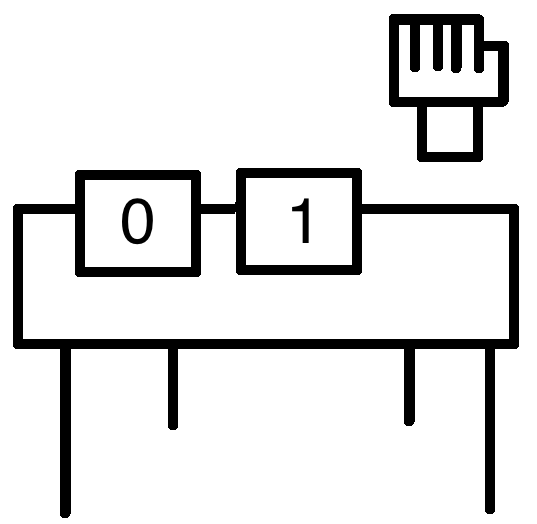
\includegraphics[width=0.4\textwidth]{figuras/blocksworld_inicial.png}
\caption[Ejemplo de estado inicial en \textit{mundo de bloques}]{Posible estado de un problema en \textit{mundo de bloques}.}
\label{blocksworld_inicial}
\end{figure}

Una acción en PDDL especifica qué debe ser cierto sobre el estado actual para
que la acción sea aplicable. 
Este conjunto comprende las \textbf{precondiciones}. Asimismo,
la acción declara qué proposiciones en el mundo cambian cuando es aplicada,
lo cual constituye sus \textbf{efectos}. Para una notación
simplificada, PDDL permite la utilización de \textbf{parámetros} en los
símbolos relacionales que describen sus precondiciones y efectos. Estos
parámetros pueden ser instanciados con cualquier objeto. Volviendo al
ejemplo anterior, un conjunto de acciones podría ser:
\begin{Verbatim}[commandchars=\\\{\},
codes={\catcode`$=3\catcode`^=7}]
(:action recoger_bloque
    :parameters (?b)
    :precondition (and (manoVacía) (libre ?b))
    :effect (and (enMano ?b) (not (manoVacía)) (not (sobreMesa ?b)))
)

(:action colocar_sobre
    :parameters (?b1 ?b2)
    :precondition (and (enMano ?b1) (libre ?b2))
    :effect (and (sobre ?b1 ?b2) (manoVacía) (not (enMano ?b1))
            (not (libre ?b2)))
)
\end{Verbatim}

Teniendo en cuenta esta especificación, el lector puede hacer el ejercicio de
generar una secuencia ordenada de acciones que resuelva este ejemplo
concreto, es decir, que conduzca desde el estado ilustrado en la Figura
\ref{blocksworld_inicial} hasta un estado en el cual los bloques estén ``apilados en
orden''. La solución se presenta a continuación. Como es costumbre, sólo se
mencionan las proposiciones verdaderas en cada estado. Se ha coloreado de azul
las nuevas proposiciones que han resultado de aplicar una acción
(\textit{adds}), y de rojo a las proposiciones que dejaron de ser ciertas en el
siguiente estado producto de la acción aplicada (\textit{deletes}).
\begin{Verbatim}[commandchars=\\\{\},
codes={\catcode`$=3\catcode`^=7}]
estado: \{sobreMesa(bloque0), {\color{red} sobreMesa(bloque1)},
         libre(bloque0), libre(bloque1), {\color{red} manoVacía}\}
\textit{acción: recoger_bloque(bloque1)}
estado: \{{\color{blue}enMano(bloque1)}, sobreMesa(bloque0),
        {\color{red} libre(bloque0)}, libre(bloque1)\}
\textit{acción: colocar_sobre(bloque1, bloque0)}
estado: \{{\color{blue}sobre(bloque1, bloque0)}, sobreMesa(bloque0),
          {\color{blue}manoVacía}, libre(bloque1)\}
\end{Verbatim}

La Figura \ref{blocksworld_final} es una representación de este estado final.

\begin{figure}[h!]
\centering
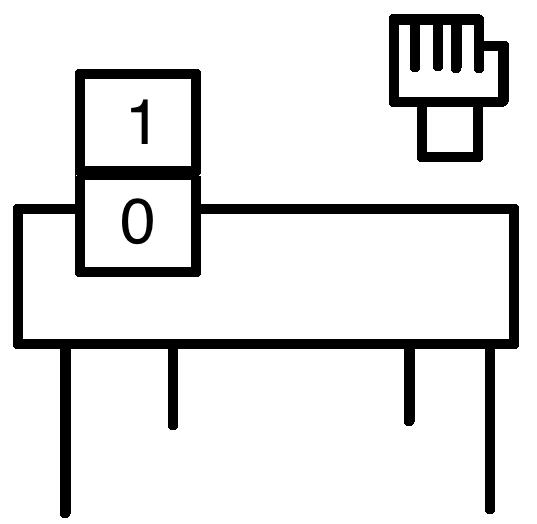
\includegraphics[width=0.4\textwidth]{figuras/blocksworld_final.png}
\caption[Estado final en \textit{mundo de bloques}]{Estado final para un problema en \textit{mundo de bloques},
luego de aplicar una secuencia de acciones al estado en la Figura
\ref{blocksworld_inicial}}
\label{blocksworld_final}
\end{figure}

En resumen, un \textbf{problema de planificación} es expresado utilizando
el lenguaje PDDL, que especifica su \textbf{estado inicial}, \textbf{acciones}
(precondiciones y efectos de cada una) y los \textbf{estados finales}.
Un \textbf{plan} es una secuencia ordenada de acciones que resuelve el problema
de planificación.

Cuando se busca resolver varias instancias de un problema general se suelen
agrupar los problemas de planificación en dominios. Dos problemas del mismo
dominio comparten el mismo conjunto de acciones, mas no necesariamente el
estado inicial o los estados meta. Por esto se dice que \textit{mundo de bloques}
es un \textbf{dominio de planificación}, y el término \textbf{problema} se refiere a
una instancia particular con estados inicial y final definidos, en
el cual pueden utilizarse las acciones del dominio al que pertenece.


Un problema de planificación en PDDL es un par $\tup{\domain,\instance}$ con
una descripción de un dominio y una instancia en el lenguaje PDDL
\citep{mcdermott:pddl,fox:pddl}.
\subsection{Complejidad en planificación}
\label{complejidad_planificacion}
Sea PLANSAT el problema de decisión que pregunta si existe un plan que
resuelve un problema de planificación dado. Según el formalismo que se ha definido
en la sección anterior,
PLANSAT es \textbf{decidible} porque el número de estados es finito:
un algoritmo basado en búsqueda desde el estado inicial que aplique
todas las acciones posibles en cada estado acabará examinando todo el espacio y
determinando si existe tal plan.

PLANSAT pertenece a la clase de complejidad PSPACE
\citep{bylander:plan-complexity}.
PSPACE es la clase de problemas que pueden ser resueltos por una máquina de
Turing determinística con una cantidad polinomial (en $n$, donde $n$ es el
tamaño del problema) de espacio en memoria. Los problemas PSPACE son, en
general, más difíciles de resolver que los problemas NP, los cuales a su vez
son problemas combinatorios complejos para los cuales se cree que no existen
soluciones generales eficientes. Como en muchos otros dominios de inteligencia
artificial, los planificadores dependen de
heurísticas de búsqueda para dar con las soluciones a problemas pequeños en un 
período de tiempo razonable.

Una restricción interesante a PLANSAT es no permitir efectos negativos en las
acciones. Si este es el caso, cualquier predicado instanciado que se haya 
agregado permanece cierto durante todo el plan, de modo que no es necesario
que el operador instanciado sea aplicado más de una vez.
Esto tiene como consecuencia que PLANSAT sin efectos 
negativos pertenezca a la clase NP \citep{ghallab:book}.

\section{Complejidad Descriptiva}
La Teoría de Complejidad Descriptiva (TCD) es un área de investigación en la
intersección entre matemáticas y las ciencias de la computación 
que estudia la teoría de complejidad desde un punto de vista matemático, 
sin utilizar modelos de computación como máquinas de Turing. La TCD surgió
cuando se demostró que la clase de complejidad NP corresponde
exactamente con la clase de problemas expresables en lógica de segundo orden
existencial \citep{fagin:spectra}. En los últimos años se ha establecido una
correspondencia entre las clases de complejidad más importantes y lenguajes
lógicos con distintos niveles de expresividad \citep{immerman:book}. En esta
sección se describen los elementos sintácticos de estos lenguajes, repasando
conceptos relevantes de la lógica, y se explica la interpretación formal de
las fórmulas construidas con estos lenguajes.

\subsection{Lenguajes}
Cada lenguaje lógico está construido a partir de un conjunto de símbolos, o
\textbf{vocabulario}.
El vocabulario se suele dividir en símbolos lógicos puros como `$\land$',
`$\exists$', etc., símbolos de puntuación como `$($' y `$)$', símbolos
relacionales, símbolos funcionales y constantes. Los símbolos lógicos y de
puntuación pertenecen a todos los lenguajes, mientras que los símbolos
relacionales, funcionales y constantes varían de un lenguaje a otro. De modo
que es conveniente definir la firma de un lenguaje como el conjunto finito de
relaciones, funciones y constantes permitidas en las fórmulas. Las firmas son
denotadas por tuplas como $\sigma=\tup{P^1,Q^2,f^1,A,B}$, que contiene dos
símbolos relacionales $P$ y $Q$ de aridades 1 y 2, respectivamente, un símbolo
funcional $f$ de aridad 1, y dos constantes $A$ y $B$.

Los símbolos funcionales de la forma $f(x) = y$ pueden representarse con una
tupla de la relación $F(x, y)$, en la que se expresa que $y$ es la imagen de
$x$, siempre y cuando se agreguen restricciones sobre $x$ y $y$ que expresen
que $f$ es una función.
Por esta razón se omiten los símbolos funcionales en lo sucesivo.

\subsubsection{Lógica de segundo orden}
Se denota con $\LPO(\sigma)$ y $\LSO(\sigma)$ a los conjuntos de todas las
fórmulas de lógica de primer y segundo orden basadas en la firma $\sigma$.
La única diferencia entre la LPO y la LSO es que en esta última se permite la
cuantificación sobre los símbolos relacionales. La fórmulas que forman parte
de LSO son descritas en la Definición \ref{lso_def}.

\begin{definition} Una fórmula pertenece a lógica de segundo orden (LSO) si y
sólo si puede construirse mediante las siguientes reglas.
\label{lso_def}
\begin{enumerate}

\item Cualquier fórmula $\LPO(\tau)$, dado $\tau\supseteq\sigma$, es una
fórmula $\LSO(\sigma)$.
\item Si $\Phi$ and $\Psi$ son fórmulas $\LSO(\sigma)$, entonces también lo
son:
 \begin{itemize}
    \item $(\Phi)$
    \item $\neg\Phi$
    \item $\Phi\land\Psi$
    \item $\Phi\lor\Psi$
    \item $\Phi\Rightarrow\Psi$
  \end{itemize}
\item Si la relación $R^a\notin\sigma$ y $\Phi$ es una fórmula $\LSO(\sigma)$,
  entonces `$(\exists R)\Phi$' y `$(\forall R)\Phi$' son fórmulas $\LSO(\sigma)$.
\end{enumerate}
\end{definition}

Las fórmulas sin variables o predicados libres se llaman \textbf{sentencias}.
Entre las fórmulas de segundo orden, en este trabajo
sólo se tratarán aquellas que sean de la forma
\[ \Phi = (\Q_1R_1^{a_1})(\Q_2R_2^{a_2})\cdots(\Q_nR_n^{a_n})\psi \]
donde cada $\Q_i \in \{\exists,\forall\}$, y
$\psi$ es una sentencia de primer orden sobre $\sigma\ \cup\ \{R_1^{a_1},\ldots,R_n^{a_n}\}$.
Esta forma es universal: todas las sentencias de segundo orden pueden llevarse
a una equivalente que cumpla con esta restricción.
Si todos los $\Q_i$ son cuantificadores existenciales, se dice que
$\Phi$ es una sentencia \textbf{existencial de segundo orden}.
La clase de todas las sentencias existenciales de segundo orden, también
llamada el \textbf{fragmento existencial de la LSO}, es denotado por \SOE. Se
define \SOA\ análogamente para el cuantificador universal,
y si existe un $k$, $1<k<n$, tal que $\Q_i=\exists$ para todo $i<k$
y $\Q_i=\forall$ para todo $i\geq k$, entonces la sentencia
pertenece al segmento \SOEA, y así sucesivamente.

\subsection{Estructuras de primer orden}
Las fórmulas lógicas son interpretadas con respecto a \textbf{estructuras de primer
orden}. Una estructura de primer orden se define sobre la firma
$\sigma=\tup{R_1^{a_1},\ldots,R_s^{a_s},\\c_1,\ldots,c_t}$, donde cada $R_i$ es
un símbolo relacional de aridad $a_i$, y cada $c_j$ es una constante. 
Una estructura de primer orden es una tupla
$\A=\tup{|\A|,R_1^\A,\ldots,R_s^\A,c_1^\A,\\\ldots,c_t^\A}$ con un universo
no vacío $|\A|$, donde cada $R_i^\A\subseteq|\A|^{a_i}$ es un subconjunto de
$a_i$-tuplas de $|\A|$, y cada
$c_j^\A\in|\A|$ es un elemento de $|\A|$.
Sin pérdida de generalidad, puede asumirse que el universo siempre es de la
forma $|\A|=\{0,1,\ldots,n-1\}$.
La TCD sólo está interesada en estructuras de universo finito, la clase de
todas las estructuras finitas de la firma $\sigma$ se denota por $\struc[\sigma]$.

Como ejemplo, sea $\sigma=\tup{E^2,s,t}$ y
$\A=\tup{|\A|,E^\A,s^\A,t^\A}$, donde $|\A|=\{0,1,2\}$,
$E^\A=\{(0,1),(1,2)\}$, $s^\A=0$ y $t^\A=2$.
Nótese que la firma $\sigma$ puede ser utilizada para describir grafos
dirigidos con vértices $s$ y $t$, y la relación $E(x, y)$ indica que hay un
arco entre los vértices $x$ y $y$. $\A$ corresponde al grafo mostrado en la
Figura \ref{grafo_simple}.

\shorthandoff{<>."}
\begin{figure}[h]
\begin{center}
\begin{tikzpicture}[shorten >=1pt, thick]%[shorten >=1pt,node distance=2cm,>=stealth',thick]
  \node [shape=circle,fill=black,inner sep=1.5pt,label=below:$s$] (q0) at (0,0) {};
  \node [shape=circle,fill=black,inner sep=1.5pt,label=below:$1$] (q1) at (2,0) {};
  \node [shape=circle,fill=black,inner sep=1.5pt,label=below:$t$] (q2) at (4,0) {};
  \path[->] (q0) edge (q1) (q1) edge (q2);
\end{tikzpicture}
\end{center}
\caption[Grafo dirigido correspondiente a una estructura \A]{El grafo dirigido que corresponde a la estructura $\A=\tup{|\A|,E^\A,s^\A,t^\A}$
donde $|\A|=\{0,1,2\}$, $E^\A=\{(0,1),(1,2)\}$, $s^\A=0$ y $t^\A=2$.}
\label{grafo_simple}
\end{figure}

La siguiente definición será de utilidad para trabajar sobre la semántica
formal.
\begin{definition}
Sea $\A \in \struc[\sigma]$ y sea $i$ una función 
$i : \text{VAR}\ \deriv |\A|$, donde \text{VAR} es el conjunto de
todas las variables.
Se dice que el par $(\A, i)$ es una \textbf{interpretación} de una fórmula de
segundo orden $\Phi \in \LSO(\sigma)$.
\end{definition}
Como ejemplo, una posible interpretación de la fórmula $\Phi =
(\exists xy) (T(x, y))$
es $(\A, i)$, para toda variable $x$, donde $i(x) = 1$ y $\A$ es la estructura ejemplo mencionada
anteriormente.
\begin{definition}
Se extiende $i$ sobre todos los términos del lenguaje. Como no hay símbolos
funcionales, sólo es necesario extender $i$ sobre las constantes. Se define
$i(a) = a^\A$ para toda constante $a \in \sigma$.
\end{definition}

\subsection{Semántica formal}
Las definiciones \ref{semantica_def} y \ref{semantica_def2} describen 
bajo qué circunstancias una fórmula $\Phi$ en
$\LSO(\sigma)$ satisface una estructura $\A$, tal como es
presentado por \cite{immerman:book}.

\begin{definition}
\label{semantica_def}
\textbf{Definición de Verdad.} Sea $\A \in \struc[\sigma]$.
Se definen inductivamente las condiciones necesarias y suficientes para que 
una fórmula $\Phi \in \LSO(\sigma)$ sea verdadera bajo la interpretación $(\A, i)$:
\[
\begin{array}{lcl}
\text{(a)} \hspace{5mm} (\A, i) \models t_1 = t_2 & \iff & i(t_1) = i(t_2)\\
\text{(b)} \hspace{5mm} (\A, i) \models R(t_1,\ldots,t_{k}) & \iff & \tup{i(t_1),\ldots,i(t_{k})} \in R^{\A}\\
\text{(c)} \hspace{5mm} (\A, i) \models \neg \Phi & \iff & (A, i) \nvDash \Phi\\
\text{(d)} \hspace{5mm} (\A, i) \models \Phi \land \Psi & \iff & (\A, i) \models \Phi \mbox{ y } (\A, i) \models \Psi\\
\text{(e)} \hspace{5mm} (\A, i) \models \Phi \lor \Psi & \iff & (\A, i) \models \Phi \mbox{ o } (\A, i) \models \Psi\\
\text{(f)} \hspace{5mm} (\A, i) \models \Phi \Rightarrow \Psi & \iff & (\A, i) \models \neg \Phi \lor \Psi\\
\text{(g)} \hspace{5mm} (\A, i) \models (\exists x) \Phi & \iff & \mbox{existe } u \in |\A| 
\mbox{ tal que } (\A, i [x:= u]) \models \Phi,\\
&&\mbox{donde } i[x:=u](y) = \left\{
     \begin{array}{lr}
       u & \mbox{si } y = x\\
       i(y) & \mbox{si } y \not= x
     \end{array}
   \right.\\
\text{(h)} \hspace{5mm} (\A, i) \models (\forall x) \Phi & \iff &
    (\A, i) \nvDash (\exists x) \neg \Phi\\
\text{(i)} \hspace{5mm} (\A, i) \models (\exists R) \Phi & \iff & \mbox{existe } R' \subseteq |\A|^k
\mbox{ tal que } (\tup{\A, R'}, i) \models \Phi,\\
&&\text{donde } \tup{\A, R'} \text{ es la estructura que extiende a $\A$ }\\
&&\text{donde $R$ se interpreta como $R'$.}\\
\text{(j)} \hspace{5mm} (\A, i) \models (\forall R) \Phi & \iff &
    (\A, i) \nvDash (\exists R) \neg \Phi\\
\end{array}
\]
\end{definition}
\begin{definition}
\label{semantica_def2}
Se dice que $\A \models \Phi$ si y sólo si para toda función $i$ se cumple $(A, i)
\models \Phi$. Se dice que $\models \Phi$, o que $\Phi$ es verdadera, si y sólo si para
toda estructura $\A \in \struc(\sigma)$ se cumple $\A \models \Phi$.
\end{definition}

Volviendo al grafo de ejemplo \A, puede verificarse mediante semántica 
formal si $\A\models\Phi$, donde $\Phi$
es una fórmula arbitraria de $\LPO(\sigma)$. A continuación se comprueba si dos
fórmulas particulares satisfacen la estructura \A. 
%No se requiere utilizar la
%noción de interpretación, pues toda sentencia $\Phi \in LSO(\sigma)$ es
%verdadera o falsa en cualquier estructura $\A \in \struc[\sigma]$.

\begin{enumerate}
\item $\A\models^?(\exists x)(E(s,x)\land E(x,t))$

Sea $i : \text{VAR} \rightarrow |\A|$ arbitraria.\\
Considere $j = i[x:=1]$.\\
Se tiene por definición \ref{semantica_def}(b) que $(\A,j) \models E(s,1)$ y que $(\A,j) \models E(1,t)$.\\
$\tup{\text{por definición \ref{semantica_def}(d)}}$\\
\mbox{\hspace{5mm} $(\A,j) \models E(s,1)\ \land E(1,t)$}\\
$\iff \tup{\text{definición \ref{semantica_def}(g)}}$\\
\mbox{\hspace{5mm} $(\A,j) \models (\exists x)(E(s,x) \land E(x,t))$}\\
$\therefore\ \A \models \Phi$, porque $i$ es arbitraria.

%\item $\A\models^?(\exists R^1)(\forall x)(E(s,x) \land R(x))$
\item La sentencia
\[ \Phi_{\textsc{2Col}} = (\exists R^1)(\forall xy)(E(x,y)\Rightarrow \neg (R(x) \iff R(y))) \]
es cierta para un grafo si y sólo si es 2-coloreable. Se comprobará formalmente
que $\A \models \Phi_{\textsc{2Col}}$ y el grafo, por tanto, es 2-coloreable.

Sea $i : \text{VAR} \rightarrow |\A|$ arbitraria.\\
Considere $R' = \{1\}$, y sea $\tup{A, R'}$ la estructura que extiende a $\A$
donde $R$ se interpreta como $R'$.\\
Se tiene por definición \ref{semantica_def}(b) que $(\tup{\A, R'},i) 
\models E(0,1)$ y que \mbox{$(\tup{\A, R'},i) \models E(1,2)$}.\\
También se tiene que $(\tup{\A, R'}, i) \models R'(1)$, 
$(\tup{\A, R'}, i) \nvDash R'(0)$, y $(\tup{\A, R'}, i) \nvDash R'(1)$.\\
$\tup{\text{por definición \ref{semantica_def}(d) y (c)}}$\\
\mbox{\hspace{5mm} $(\tup{\A, R'}, i) \models E(0,1) \land E(1,2) \land \neg
R'(0) \land R'(1) \land \neg R'(2)$}\\
$\iff \tup{\text{operadores de la lógica proposicional}}$\\
\mbox{\hspace{5mm} $(\tup{\A, R'}, i) \models (E(0,1) \Rightarrow \neg R(0)
\iff R(1))\ \land$} \\ 
\mbox{\hspace{30mm} $(E(1,2) \Rightarrow R(1) \iff \neg R(2))$}\\
$\iff \tup{\text{definición \ref{semantica_def}(h)}}$\\
\mbox{\hspace{5mm} $(\tup{\A, R'}, i) 
\models (\forall xy)(E(x, y) \Rightarrow \neg(R'(x) \iff R'(y)))$}\\
$\iff \tup{\text{definición \ref{semantica_def}(i)}}$\\
\mbox{\hspace{5mm} $(\A, i) 
\models (\exists R^1)(\forall xy)(E(x, y) \Rightarrow \neg(R(x) \iff R(y)))$}\\
$\therefore\ \A \models \Phi$, porque $i$ es arbitraria.
\end{enumerate}

La Figura \ref{grafo_coloreado} muestra una 2-coloración del grafo correspondiente a \A
\ inducida por $R$.

\begin{figure}[h]
\begin{center}
\begin{tikzpicture}[shorten >=1pt, thick]%[shorten >=1pt,node distance=2cm,>=stealth',thick]
  \node [shape=circle,fill=black,inner sep=1.5pt,label=below:$s$] (q0) at (0,0) {};
  \node [shape=circle,fill=blue,inner sep=1.5pt,label=below:$1$] (q1) at (2,0) {};
  \node [shape=circle,fill=black,inner sep=1.5pt,label=below:$t$] (q2) at (4,0) {};
  \path[->] (q0) edge (q1) (q1) edge (q2);
\end{tikzpicture}
\end{center}
\caption[Grafo dirigido coloreado por una relación]{El grafo dirigido de la Figura \ref{grafo_simple}, coloreado
utilizando la relación $R$. Los nodos para los cuales $R$ es verdadera son
azules, los otros son negros.}
\label{grafo_coloreado}
\end{figure}

\subsection{Abreviaciones sintácticas}
Con frecuencia es necesario cuantificar sobre una función de aridad $k$ ($f^k$)
en lugar de una relación. Esto puede hacerse cuantificando sobre una relación de
aridad $k+1$ ($F^{k+1}$) y agregando fórmulas de primer orden que garanticen
que $F$ represente a $f$. Por ejemplo, una función parcial unaria $f$ puede ser
representada por la relación binaria $F$ y la fórmula
\[ \psi_{fun} = (\forall xyy')(F(x, y) \land F(x, y') \Rightarrow y = y'). \]

De igual forma, se puede representar una función inyectiva añadiendo a las
proposiciones la fórmula anterior más

\[ \psi_{iny} = (\forall xx'y)(F(x, y) \land F(x', y) \Rightarrow x = x'). \]

Finalmente, si es necesario que la función sea total debe agregarse
\[ \psi_{tot} = (\forall x)(\exists y)(F(x, y)). \]

Se utilizarán las abreviaciones siguientes para denotar distintos
tipos de funciones:

\begin{tabular}{ll}
$(\exists F \in \text{Fun})$ & función total\\
$(\exists F \in \text{Inj})$ & función total inyectiva\\
$(\exists F \in \text{PFun})$ & función parcial\\
$(\exists F \in \text{PInj})$ & función parcial inyectiva\\
\end{tabular}

\subsection{Clases de complejidad}
El ejemplo anterior evidencia que una sentencia puede describir una colección
de estructuras discretas finitas (como grafos dirigidos) que satisfacen
una cierta propiedad (como 2-colorabilidad). 

En la TCD, un problema de decisión corresponde a una clase de estructuras de
primer orden que satisface a una sentencia, y por lo tanto los problemas de
decisión pueden ser \textbf{modelados con fórmulas lógicas de segundo orden}.
El trabajo de \cite{fagin:spectra} estableció que todos los problemas de
decisión en NP pueden ser caracterizados por la clase de estructuras que
satisfacen una sentencia de segundo orden existencial, es decir,
$\text{NP}=\SOE$.

Esta lista muestra los resultados más importantes de la TCD sobre la
caracterización de clases de complejidad \citep{immerman:book}:
\begin{itemize}
\item Espacio logarítmico no determinista (NL) es igual a la \LPO\ extendida con
un operador de clausura transitiva.
\item Espacio polinomial (P) es igual a las sentencias Horn de segundo orden
(SO-Horn).
\item Tiempo polinomial no determinista (NP) es igual a \SOE.
\item Co-NP es igual a \SOA.
\item La jerarquía de tiempo polinomial (PH) es igual a la lógica 
de segundo orden (\LSO) completa.
\item Espacio polinomial (PSPACE) es igual a la lógica de segundo orden
extendida con un operador de clausura transitiva.
\end{itemize}

%A transitive-closure operator is a \emph{syntactic construct}
%whose interpretation coincides with the transitive closure of
%a relation. Thus, it is not surprising that NL equals FO(TC)
%because checking the existence of a path from node $s$ to
%node $t$ in a digraph with designated vertices $s$ and $t$ is
%NL-complete \cite{sipser:book}, and this property
%holds whenever $s$ is related to $t$ in the transitive closure
%of the edge relation.

\section{Modelación de problemas}
\label{modelacionproblemas}
Consideremos, por ejemplo, el problema de satisfacibilidad
proposicional (SAT). Una instancia de SAT es una fórmula en forma normal
conjuntiva con $m$ cláusulas sobre $n$ variables proposicionales, donde una
cláusula es un subconjunto de literales positivos y negativos. 
Sean $P^2$, $N^2$ dos símbolos relacionales que describen las ocurrencias
positivas y negativas de los literales en las cláusulas: $P(x, y)$ expresa que
la variable $x$ aparece positiva en la cláusula $y$. Respectivamente, $N(x, y)$ expresa
su ocurrencia negativa.
Por ejemplo, $(p\lor \neg q\lor r)\land(\neg p\lor \neg r)\land(\neg p\lor q)$
es codificado como $\A=\tup{|\A|,N^\A,P^\A}$, donde $|\A|=\{0,1,2\}$,
$N^\A=\{(1,0),(0,1),(2,1),(0,2)\}$ y $P^\A=\{(0,0),(2,0),(1,2)\}$.

La existencia de una asignación de valores de verdad a las variables que
satisfaga una fórmula en forma normal conjuntiva (CNF) puede ser expresada con la
sentencia \SOE $\Phi_\SAT$:\footnote{Esta sentencia
asume que $m\geq n$. En caso contrario, se debe añadir cláusulas tautológicas a
la fórmula en CNF.}
\[ (\exists T^1)(\forall y)(\exists x)[(P(x,y)\land T(x))\lor(N(x,y)\land\neg T(x))] \]

La fórmula puede leerse como: existe una asignación de valores de verdad $T$
tal que en toda cláusula hay al menos una variable que cumple una de las
siguientes condiciones:
\begin{enumerate}[--]
\item la variable aparece positiva en la cláusula y está asignada a verdadero,
i.e. $T(x)$
\item la variable aparece negativa en la cláusula y está asignada a falso, i.e.
$\neg T(x)$
\end{enumerate}

Nótese que $T$ es un \textit{certificado}, pues muestra cuál es la asignación 
de variables necesaria para que la fórmula en CNF sea cierta.

En el Apéndice \ref{apendiceA} se encuentran las fórmulas correspondientes a
varios problemas NP, como camino hamiltoniano dirigido y colorabilidad de
grafos, entre otros.

% Chapter 2

\chapter{Traducción de problemas NP}
\label{Chapter2}
\lhead{Capítulo 2. \emph{Traducción de problemas NP}}
Este capítulo describe el diseño de una herramienta capaz de transformar una
descripción de un problema en lógica de segundo orden 
en un problema de planificación de clase de complejidad equivalente. 
Primero se presenta una perspectiva a alto nivel de lo que de

\section{Perspectiva general}
\begin{figure}[h!]
\centering
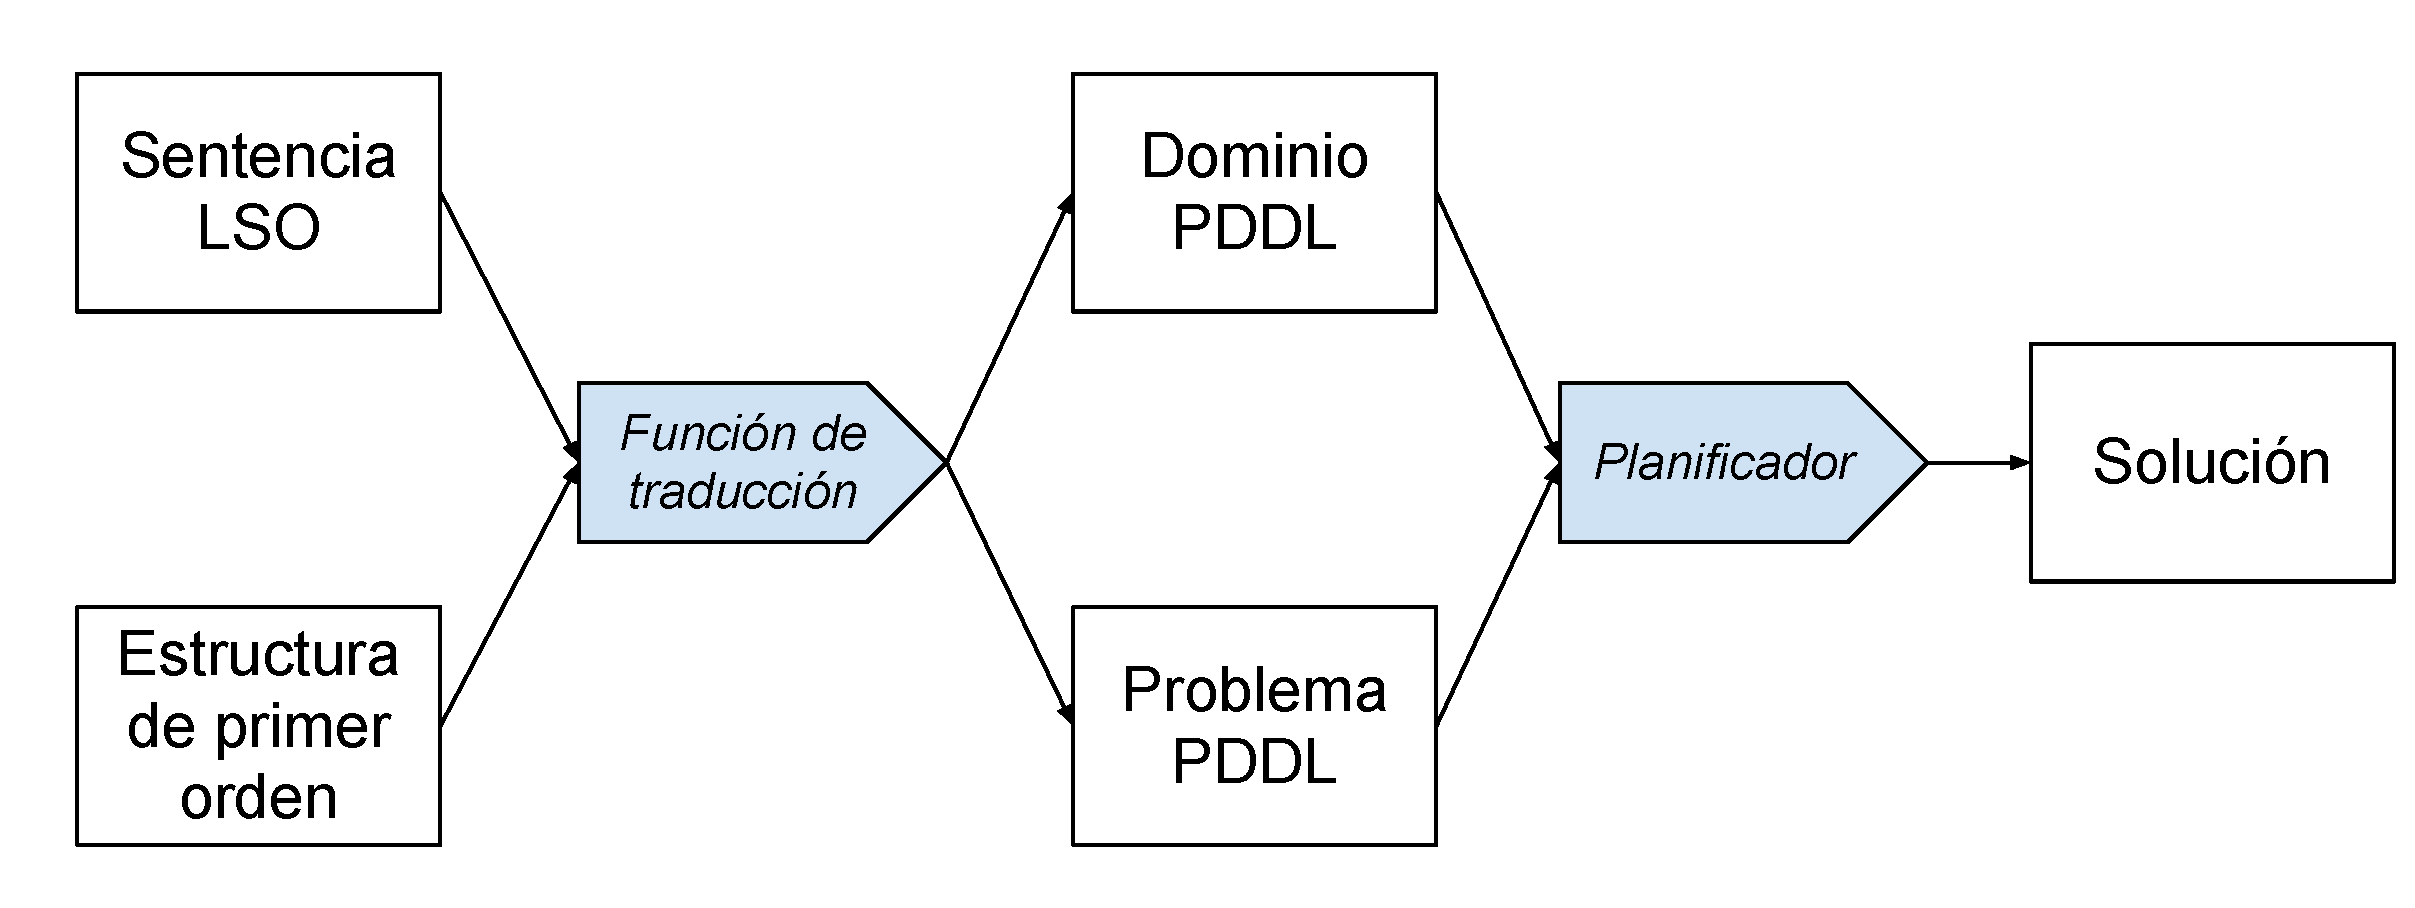
\includegraphics[width=\textwidth]{figuras/esquema_herramienta.pdf}
\caption{Esquema de operación de la herramienta}
\label{esquema_herramienta}
\end{figure}

\section{Diseño del lenguaje}

\subsection{Gramática}
\begin{alignat*}{1}
\sofbf\   & \deriv\ \lpar \SOExists\ \lpar \listrel \rpar\ \sofbf \rpar \\
          & \deriv\ \lpar \SOForall\ \lpar \listrel \rpar\ \sofbf \rpar \\
          & \deriv\ \pofbf \\[1em]
\listrel\ & \deriv\ \rel\ \integer\ \listrel\ |\ \rel\ \integer \\
          & \deriv\ \rel\ \tipof\ \listrel\ |\ \rel\ \tipof\ \\[1em]
\tipof\   & \deriv\ \fun\ |\ \pfun\ |\ \inj\ |\ \pinj\ \\[1em]
\pofbf\   & \deriv\ \lpar \rel\ \listvar \rpar \\
          & \deriv\ \lpar \NOT\ \pofbf \rpar \\
          & \deriv\ \lpar \AND\ \listpofbf \rpar \\
          & \deriv\ \lpar \OR\ \listpofbf \rpar \\
          & \deriv\ \lpar \IMPLIES\ \pofbf\ \pofbf \rpar \\
          & \deriv\ \lpar \Exists\ \lpar \listvar \rpar\ \pofbf \rpar \\
          & \deriv\ \lpar \Forall\ \lpar \listvar \rpar\ \pofbf \rpar \\[1em]
\listvar\ & \deriv\ \var\ \listvar\ |\ \var \\[1em]
\end{alignat*}

\section{Reducción base}
\subsection{Reducción del dominio}
\subsection{Reducción del problema}

\section{Propiedades formales}
Las propiedades más importantes a considerar en la herramienta son solidez,
completitud y garantía de complejidad. Que la función de traducción sea sólida
y completa significa que ella realmente implementa una reducción entre problemas de
decisión, mientras que la garantía de complejidad se refiere al tiempo
requerido para computar la reducción y la complejidad de decidir la existencia
de un plan en el problema generado. En esta sección se demuestra que la 
herramienta es una reducción en tiempo
polinomial del problema NP expresado por $\Phi$ a un fragmento de planificación
que es decidible en NP.

Como se ha mencionado en la sección \ref{complejidad_planificacion}, 
se sabe que verificar la existencia de un plan para 
problemas de planificación
sin efectos negativos está en NP \citep{bylander:plan-complexity}. La prueba
depende del hecho de que un plan óptimo no necesita repetir acciones, y por lo
tanto es de tamaño lineal. Puede extenderse esta noción: si todas las acciones que
agregan efectos negativos pueden ser aplicadas a lo sumo una vez, verificar la
existencia de un plan sigue estando en NP, pues el tamaño del plan no podrá ser
mayor al número de acciones.

\begin{definition}
Un problema de planificación $P = \tup{C, A, I, F}$ es de tipo
\textit{máximo-1} si y sólo si las acciones pueden ser particionadas en $A =
A_0 \cup A_1$, donde:
\begin{itemize}
\item Ninguna de las acciones de $A_0$ tiene efectos negativos, es decir,
$(\forall a \in A_0) (del(a) = \emptyset)$.
\item Todas las acciones de $A_1$ tienen una precondición que no es añadida por
ninguna acción, y que es borrada apenas $a$ es ejecutada, es decir, 
$(\forall aa' \in A_1)\ (\exists p \in pre(a) \cap del(a))\ (p \not\in add(a'))$
\end{itemize}

El conjunto de todos los problemas \textit{máximo-1} se denota como STRIPS-1.
\end{definition}

%! ???
Ahora considere la función de \emph{instanciación} $\ground$ que transforma el par
$\tup{\domain,\instance}$ de un dominio y problema PDDL en un problema STRIPS
$P = \ground(\domain, \instance)$. Para un $\domain$ fijo, la función
$\instance\leadsto\ground(\domain, \instance)$ corre en un tiempo polinomial
$\O(\|\instance\|^k)$ para algún $k$ que sólo depende de $\domain$; de hecho,
$k$ es la máxima aridad de un predicado o acción en el dominio.

De manera similar, la función de traducción $\insred$ corre en tiempo
polinomial en el tamaño de la estructura $\A$, pero exponencial sobre la aridad
más grande de un cuantificador de segundo orden existencial en $\Phi$. De este
modo, la función $f_{\sigma,\Phi}:\struc[\sigma]\rightarrow\text{STRIPS}$
definida por 
\[ f_{\sigma,\Phi}(\A) = \ground(\domred(\sigma,\Phi),\insred(\sigma,\Phi,\A)) \]
es una función en tiempo polinomial que asigna a las $\sigma$-estructuras un
problema instanciado STRIPS. Esta función es una reducción, tal como es
demostrado por

\begin{theorem}
La función $f_{\sigma, \Phi}$ es una reducción en tiempo polinomial del
problema de decisión inducido por $\Phi$ a STRIPS-1.
\end{theorem}

\begin{proof}
Se quiere demostrar que
$\A\models(\exists R_1^{a_1})\cdots(\exists R_k^{a_k})\psi$ si y sólo si
existe un plan que consigue la condición $\FT[\psi]$. La prueba es inductiva
sobre la sentencia de primer orden $\psi$. Se demostrará que para toda subformula 
$\theta$ de $\psi$, y toda interpretacion $(\A,i)$ de $\A$:

\[ (\A,i) \models \theta(\overline{X}) \iff \text{existe un plan para } \FT[\theta](\overline{X}) \]

Por implicación mutua. Primero se prueba
\[ (\A,i) \models \theta(\overline{X}) \Rightarrow \text{existe un plan para } \FT[\theta](\overline{X}) \]

\begin{tabular}{ll}
\multirow{2}{*}{Caso base: $\theta$ es un literal, $\theta = P(\overline{X})$}\\
\multirow{2}{*}{Caso $P(\overline{X})$ $\in$ $\sigma$}
\end{tabular}

\begin{itemize}
		\item Caso base: $\theta$ is a literal. $\theta = P(X)$ 
		
		Prueba por casos:
			\begin{itemize}
				\item Caso 0: $P(\overline{X})$ $\epsilon$ $\sigma$
				
				\begin{tabular}{@{}p{1mm}p{1mm}p{11cm}}	
						& & $\A \models P(\overline{X})$\\
						$\eq$ & & $<(A,i)$ es una interpretacion de $\A>$ \\
						& & $(A,i) \models P(\overline{X})$ \\
						$\eq$ & & $<$Definicion de interpretacion$>$\\
						& & $i(\overline{X})$ $\epsilon$ $P^{\A}$\\
						$\Rightarrow$ & & $<$ La situacion inicial (Init) consiste de fluents describiendo el valor de 
									  verdad de todas las relaciones en $\A$$>$\\
						& & $P(\overline{X})$ $\epsilon$ $Init$ \\
						$\eq$ & & $<$ Hy un plan de cero pasos para $\theta(\overline{x})>$\\
						& & $\FT[\theta](\overline{X})$ tiene solucion
					\end{tabular}
					
					
				\item Caso 1: $P(\overline{X})$ $\epsilon$ $\Phi$
				
					  Falta
			\end{itemize}
			
		\item Caso inductivo:
			\begin{itemize}
				\item Caso 0: $\theta = \neg P(\overline{X})$ (Como esta definido en el paper la negacion esta solo en los literales)
				
				\begin{tabular}{@{}p{1mm}p{1mm}p{11cm}}	
						& & $\A \models \neg P(\overline{X})$\\
						$\eq$ & & $<(A,i)$ es una interpretacion de $\A>$ \\
						& & $(A,i) \models \neg P(\overline{X})$ \\
						$\eq$ & & $<$Definicion de interpretacion$>$\\
						& & $i(\overline{X})$ $\epsilon$ ${\neg P}^{\A}$\\
						$\Rightarrow$ & & $<$ La situacion inicial (Init) consiste de fluents describiendo el valor de 
									  verdad de todas las relaciones en $\A$ (La negacion de un literal es tomado como
									  un fluent nuevo)$>$\\
						& & $P(\overline{X})$ $\epsilon$ $Init$ \\ 
						$\eq$ & & $<$ Hy un plan de cero pasos para $\theta(\overline{x})>$\\
						& & $\FT[\theta](\overline{X})$ tiene solucion
				\end{tabular}
					
				\item Caso 1: $\theta = \psi \land \psi'$ (Logical And)
					  
					  Hipotesis inductiva:
					 	\begin{itemize}
					 		\item $(A,i) \models \psi \eq$ hay un plan para $\FT[\psi] = \pi$
							\item $(A,i) \models \psi' \eq$ hay un plan para $\FT[\psi'] = \pi'$
					 	\end{itemize}
				
					\begin{tabular}{@{}p{1mm}p{1mm}p{11cm}}	
					 	& & $\A \models \psi \land \psi'$\\
						$\eq$ & & $<(A,i)$ es una interpretacion de $\A>$ \\
						& & $(A,i) \models \psi \land \psi'$ \\
						$\eq$ & & $<$ Semantica de Primer orden $>$\\
						& & $(A,i) \models \psi \land (A,i) \models \psi'$ \\
						$\eq$ & & $<$Hipotesis inductiva$>$\\
						& & $\FT[\psi] = \pi \land \FT[\psi'] = \pi'$\\
						$\Rightarrow$ & & $<$ Operator $ prove\_and\_id >$\\
						& & $\FT[\theta](\overline{X})$ tiene solucion
					\end{tabular}
				\item Caso 2: $\theta = \psi \lor \psi'$ (Logical Or)
					  
					  Hipotesis inductiva:
					 	\begin{itemize}
					 		\item $(A,i) \models \psi \eq$ hay un plan para $\FT[\psi] = \pi$
							\item $(A,i) \models \psi' \eq$ hay un plan para $\FT[\psi'] = \pi'$
					 	\end{itemize}
				
					\begin{tabular}{@{}p{1mm}p{1mm}p{11cm}}	
					 	& & $\A \models \psi \lor \psi'$\\
						$\eq$ & & $<(A,i)$ es una interpretacion de $\A>$ \\
						& & $(A,i) \models \psi \lor \psi'$ \\
						$\eq$ & & $<$ Semantica de Primer orden $>$\\
						& & $(A,i) \models \psi \lor (A,i) \models \psi'$ \\
						$\eq$ & & $<$Hipotesis inductiva$>$\\
						& & $\FT[\psi] = \pi \lor \FT[\psi'] = \pi'$\\
						$\eq$ & & $<$ Operator $ prove\_or\_id$ twice, idempotencia del $\lor$ $>$\\
						& & $\FT[\theta](\overline{X})$ tiene solucion
					\end{tabular}
					
				\item Caso 3: $\theta = \exists x$ $ \psi(\overline{y},x)$ (Exists)
					  
					  Hipotesis inductiva:
					 	\begin{itemize}
					 		\item $(A,i) \models \psi(\overline{y},x)$ hay un plan $\pi$ para $\FT[\psi(\overline{y},x)] (\overline{y},x)$
					 	\end{itemize}
				
					\begin{tabular}{@{}p{1mm}p{1mm}p{11cm}}	
					 	& & $A \models \exists x$ $ \psi(\overline{y},x)$\\
						$\eq$ & & $<(A,i)$ es una interpretacion de $\A>$ \\
						& & $(A,i) \models \exists x$ $ \psi(\overline{y},x)$ \\
						$\eq$ & & $<$ Semantica de Primer orden $>$\\
						& & $(A,i) \models \psi(\overline{y},x)$ \\
						$\eq$ & & $<$Hipotesis inductiva$>$\\
						& & $\FT[\psi] = \pi \lor \FT[\psi'] = \pi'$\\
						$\eq$ & & $<$ Operator $ prove\_exists >$\\
						& & $\FT[\exists x$ $ \psi(\overline{y},x)](\overline{y})$ tiene solucion
					\end{tabular}

			\end{itemize}
		
	\end{itemize}
\end{proof}

% Chapter 4

\chapter{Traducción de problemas PH}
\label{Chapter3}
\lhead{Capítulo 3. \emph{Traducción de problemas PH}}

%In this approach, a decision problem $\Pi$ in NP is encoded as a
%second-order existential (\SOE) formula $\Phi$ while a particular
%instance is encoded as first-order structure $\A$ in a way that
%$\A\models\Phi$ iff the instance encoded by $\A$ satisfies belongs to $\Pi$.
%This is a general and feasible idea as it is known that \SOE
%captures the class NP \cite{immerman:book}.
%The pair $\tup{\Phi,\A}$ is then fed into a (software) tool that
%outputs a \STRIPS problem $P$ that has a solution (plan) iff $\A\models\Phi$,
%thus allowing the utilization of the current planning technology
%to automatically solve the problems in NP that are expressed as
%second-order formulas.
%Moreover, the problem $P$ is not an arbitrary \STRIPS problem but
%one that can be solved in polytime by a non-deterministic
%Turing machine, thus guaranteeing that the whole approach is not
%an overkill from the standpoint of complexity theory.
%Furthermore, the function $\tup{\Phi,\cdot}:\struc\mapsto\STRIPS$ 
%that is implemented by the tool for fixed $\Phi$ and that maps
%first-order structures $\A$ into \STRIPS problems $P$ is computable
%in polynomial time and thus corresponds to a genuine \emph{polytime many-one reduction}
%from $\Pi$ into \STRIPS.

%Since it is known that other (bigger) complexity classes are also
%captured in second-order logic, PMB left as an open issue the
%development of a tool capable of targeting such classes.
Este capítulo describe la extensión de la herramienta desarrollada en este
trabajo para la traducción de problemas de decisión pertenecientes a la clase de
complejidad de la jerarquía polinomial, PH, los cuales son capturados por la lógica de
segundo orden. En primer lugar se habla brevemente sobre la complejidad de esta
clase de problemas. Luego se presenta, mediante ejemplos, una traducción alternativa a la
expuesta en el capítulo anterior que permite traducir cualquier problema
expresado en lógica general de segundo orden a un problema de planificación
automática.

\section{Complejidad}

Al contrario que en el caso de NP,
esta vez no se ofrecen garantías de complejidad sobre la extensión de la
reducción: los problemas \STRIPS generados por ella en general no serán
solucionables en tiempo polinomial no determinístico.
Esto se debe a que los problemas de esta clase sólo admiten planes
de longitud exponencial en el peor caso ya que PH contiene, además de a NP, las
clases coNP y $\Sigma^p_k$ para todo $k\geq 1$. La clase $\Sigma_p^2$, por
ejemplo, es igual a $P^{NP}$, la clase de problemas resolubles en tiempo
polinomial contando un oráculo para resolver problemas NP.

Una característica de NP es la 
disponibilidad de un \textit{certificado} que valida en tiempo polinomial una
respuesta al problema de decisión: tal garantía no es ofrecida en estas clases
superiores.
De este modo, los problemas de planificación que produce la reducción son
cortos, pues pueden ser codificados por las traducciones de estructuras finitas
$\A$, pero sus soluciones son, potencialmente, muy largas.

%The consequences of having small problems with long solutions
%are several. Among others, such problems pose a difficult
%challenge on the current state-of-the-art planners which are
%all based on heuristic search. In particular, heuristics functions
%that are based on the delete relaxation or that do not take into
%account that the same action may be applied a large (i.e., exponential)
%number of times will probably fail at being effective for guiding
%the search.
%Surprisingly, the current best SAT-based planner, the planner M,
%is able to solve some of these challenging
%\STRIPS problems for which forward-search planners like LAMA'11
%are totally lost. Yet, more surprisingly, LAMA'11 is quite
%superior to M in one of the tested domains (more about this below).

%\section{Capturing \PH in Second-Order Logic}
%
%NP is captured by \SOE \cite{fagin:spectra}.
%This result means that any decision problem $\Pi$ in NP can be
%characterized by a second-order formula $\Phi$ that looks like
%\begin{equation}
%\label{eq:soe}
%\Phi = (\exists R_1^{a_1})\cdots(\exists R_n^{a_n})\psi
%\end{equation}
%where each symbol $R_i^{a_i}$ is a existentially-quantified relation
%of arity $a_i$, and $\psi$ is an arbitrary first-order sentence 
%over a vocabulary containing $\{R_1^{a_1},\ldots,R_n^{a_n}\}$.
%That is, $\Pi$ is the set of instances (words in a language)
%that when encoded as structures $\A$ satisfy the formula $\Phi$.

coNP es la clase complementaria a NP, y es capturada por la lógica \SOA\ 
que contiene fórmulas que se apegan a la Ecuación \ref{eq:soa}:
\begin{equation}
\label{eq:soa}
\Phi = (\forall R_1^{a_1})\cdots(\forall R_n^{a_n})\psi
\end{equation}

En general, $\Sigma^p_k$ es capturada por fórmulas cuya estructura contiene $k$
bloques alternantes de cuantificadores, empezando con los existenciales. Por
ejemplo, $\Sigma^p_2=\SOEA$ corresponde a fórmulas de la forma:
\begin{equation}
\Phi = (\exists R_1^{a_1}) \cdots (\exists R_n^{a_n}) 
       (\forall S_1^{a'_1}) \cdots (\forall S_m^{a'_m})
       \psi
\end{equation}

%Como \PH $ = \bigcup_{k\geq 1}\Sigma^p_k$ y es caracterizada por fórmulas
%arbitrarias de lógica de segundo orden \cite{immerman:book}, la extensión
%deberá manejar estas fórmulas
%
%the extended tool we sought must target such formulas
%instead of the more restricted \SOE formulas.
%On the other hand, we know that $\PH\subseteq\PSPACE$, the
%decision problem for \STRIPS is \PSPACE-complete and there
%are no known syntactic restrictions on \STRIPS that place
%its decision problem in \PH. Thus, the new tool will focus
%on generating (unrestricted) \STRIPS problems.

Considere ahora la fórmula $\Phi=(\forall R^1)\psi$
y una estructura $\A$ con universo $|\A|$.
Se dice que $\Phi$ es válida en $\A$ si y sólo si para toda
interpretación $R^\A$ de $R$, donde $R^\A \subseteq |\A|$, se tiene
$\tup{\A,R^\A}\models\psi$. Como existen $2^{\|\A\|}$ interpretaciones
distintas de $R$, una demostración de $\A\models\Phi$ puede ser de
\textbf{tamaño exponencial}. Por ejemplo, si $\Phi_{\UNSAT}$ denota el problema
complementario a satisfacibilidad proposicional, entonces una prueba de que la
estructura $\A$ es no satisfacible es de tamaño exponencial, dado que debe
considerar todos los valores de verdad para las variables proposicionales de
$\A$. Por ello, las soluciones para el problema de planificación $P$ generado
por el par $\tup{\Phi_\UNSAT,\A}$ codifican tales pruebas y son de tamaño
exponencial.

\section{Traducción a \STRIPS}

\subsection{Sistema de tipos}
Antes de extender la traducción a \PH es conveniente agregarle un sistema
sencillo de tipos.

Sea $\t^*$ un sistema, creado a partir de un conjunto finito 
$\t=\{\mathbf{t}_0,\mathbf{t}_1,\ldots,\mathbf{t}_N\}$
de \textbf{tipos atómicos}, donde $\t^*$ es el conjunto más pequeño que
contiene $t$ y todos los tipos de la forma $t=t'\times t''$
para $t'\in\t^*$ y $t''\in\t$.

La idea es que a cada objeto en una estructura de primer orden le es asignado
un tipo atómico, siendo $\mathbf{t}_0$ el tipo que contiene a todos los
objetos.
Los tipos se utilizan para restringir las iteraciones sobre las
cuantificaciones de primer y segundo orden en las fórmulas.
Por ejemplo, $(\forall x\in t)$ se refiere a una cuantificación de primer orden
sobre todos los objetos de tipo $t\in\t$, mientras que
$(\forall R^t)$ se refiere a un predicado de segundo orden universalmente
cuantificado $R$ de tipo $t\in\t^*$.
La única restriccion que se exige es que los tipos complejos en 
$\t^*\setminus\t$ sólo aparezcan en cuantificaciones de segundo orden.

Considere una fórmula general \LSO\ de la forma
\begin{equation}
\Phi = (\Q_1R_1^{t_1})(\Q_2R_2^{t_2})\cdots(\Q_nR_n^{t_n})\psi
\end{equation}
donde cada $\Q_i\in\{\exists,\forall\}$ es un cuantificador de segundo orden,
$R_i$ es un símbolo relacional de tipo $t_i\in\t^*$,
y $\psi$ es una sentencia de primer orden.

Sea $\A$ una estructura de primer orden en $\struc[\sigma]$.
Se muestra cómo generar un problema de planificación $P$ que tiene solución si
y sólo si $\A\models\Phi$.
%Further, let $\A$ be a first-order structure over the
%vocabulary of $\psi$.

Según la traducción descrita en el capítulo 2, 
$P$ tiene condiciones de la forma $\FT[\theta]$
para cada subfórmula $\theta$ de $\psi$ y con parámetros que corresponden a las
variables libres de $\theta$. Por ejemplo, si $\Phi$ es la fórmula para SAT:
\begin{alignat*}{1}
\Phi_\SAT &= (\exists T^\text{Var})\psi_\SAT \,, \\
\psi_\SAT &= (\forall y\in \text{Cls})(\exists x\in\text{Var}) \notag \\
          &\quad\quad\quad\quad
               [(P(x,y) \land T(x)) \lor (N(x,y) \lor \neg T(x))]
\end{alignat*}
donde `Var' y `Cls' son los tipos para variables y cláusulas,
entonces existe una condición $\FT[\theta]$ con parámetros
$\tup{x,y}$ para la subfórmula $\theta(x,y)=N(x,y)\lor\neg T(x)$.
En $\psi_\SAT$, las relaciones $P(x,y)$ y $N(x,y)$ denotan
que la variable $x$ aparece positiva o negativa, respectivamente, en la
cláusula $y$.
%the clause $y$; these relations are fixed for a given SAT instance
%and their interpretation is given in the structure $\A$ that
%encodes the instance.
%Por otro lado, la relación existencialmente cuantificada $T$ codifica 
%On the other hand, the existentially-quantified relation $T$
%encodes the sought model in a way that $T(x)$ is true iff the
%variable $x$ is assigned the truth-value true.

%The problem $P$ has actions for choosing the valuation $T$,
%that is represented by fluents of the form `$\texttt{T}(?x)$'
%and `$\texttt{not\_T}(?x)$', and actions for building a
%proof for $\psi_\SAT$ that are designed to work by following
%the recursive structure of $\psi_\SAT$.
%The goal of the problem is defined as the single fluent
%$\FT[\psi_\SAT]$ which has no parameters as $\psi_\SAT$
%is assumed to be a sentence.

%\smallskip

%In our approach, we make use of the same fluents that denote
%the validity of subformulas and the quantified relations.
\subsection{Traducción del operador \texttt{so-forall}}
Para la extensión de la herramienta, debe tenerse en cuenta cómo las relaciones
cuantificadas se construyen y se intercalan con las pruebas de las subfórmulas.
Este problema no surge con los problemas \SOE, debido a que hay una sola
interpretación que construir para cada fórmula existencialmente cuantificada,
pero para fórmulas generales es necesario construir e intentar probar varias
interpretaciones diferentes.
Para aclarar este punto, considere la fórmula para UNSAT, que contiene una
relación unaria $T$ cuantificada universalmente:

\begin{alignat*}{1}
\Phi_\UNSAT &= (\forall T^\text{Var})\psi_\UNSAT \\
\psi_\UNSAT &= (\exists y\in\text{Cls})(\forall x\in\text{Var}) \\
            &\quad\quad\ [(\neg P(x,y) \lor \neg T(x))\land(\neg N(x,y)\lor T(x))]
\end{alignat*}
Esta fórmula expresa que para toda relación $T$ sobre variables
proposicionales, existe una cláusula $y$ tal que para cada variable $x$, si $x$
aparece positiva en $y$, $x$ es falsa, y si $x$ aparece negativa en $y$, $x$ es
verdadera.
UNSAT se puede traducir automáticamente a \STRIPS considerando acciones que
\textbf{iteran} sobre todas las posibles relaciones $T$, y acciones para
obtener la condición $\FT[\psi_\UNSAT]$ para cada una de estas $T$.

Como $T$ es una relación unaria, hay $2^n$ relaciones distintas en $n$
variables. Cada relación puede ser codificada con una cadena binaria
de tamaño $n$ (un bit por variable) tal que el $i$-ésimo bit es 1 si y sólo si
la $i$-ésima variable $x_i$ pertenece a $T$. Luego, iterar sobre todas las
relaciones es equivalente a iterar sobre todas las cadenas binarias de tamaño
$n$: puede hacerse empezando con la relación vacía, que corresponde a
`0\ldots00', y sucesivamente ``sumando 1 a la cadena'' hasta llegar a `1\ldots11'.

La Figura \ref{fig:unsat} muestra 5 acciones que realizan la iteración en el
caso de $\Phi_\UNSAT$: estas
acciones utilizan como condiciones adicionales $\FT[\Phi_\UNSAT]$,
\texttt{necesita-}$\FT[\Phi_\UNSAT]$, `Marcador-T($x$)', `VarPrimera-T($x$)',
`VarSuc-T($x,y$)' y `VarÚlt-T($x$)'. Los últimos tres tipos de condición son
estáticos: se agregan al estado inicial e implementan un orden estático de los
objetos que se refieren a variables proposicionales.

Se describirá brevemente cómo funciona la iteración.
El estado inicial contiene las condiciones estáticas que definen a los tipos
Var y Cls, y las relaciones binarias 
$N(x,y)$ y $P(x,y)$, más la condición
\texttt{necesita-}$\FT[\Phi_\UNSAT]$. El estado final contiene solamente la
condición $\FT[\Phi_\UNSAT]$.
Inicialmente, la única acción aplicable es A1, que interpreta a $T$ como la
relación vacía y agrega la condición \texttt{necesita-}$\FT[\psi_\UNSAT]$.

Esta condición activa a las acciones para construir una prueba de $\psi_\UNSAT$
para el $T$ actual. Una vez que $\psi_\UNSAT$ ha sido probada, se agrega la
condición $\FT[\psi_\UNSAT]$.

Cuando $\psi_\UNSAT$ es demostrado, A2 se convierte en la única acción
aplicable y \textbf{borra la condición} $\FT[\psi_\UNSAT]$, agregando
Marcador($x$) para la primera variable en el orden estático.
Luego de A2, A3 debe ser aplicado, y cambia $T$ del modelo que corresponde a
0\ldots00 al modelo que corresponde a 0\ldots01. También agrega
\texttt{necesita-}$\FT[\psi_\UNSAT]$, lo que exige una demostración de
$\psi_\UNSAT$ para la nueva $T$.

La iteración procede de manera similar hasta demostrar $\psi_\UNSAT$ para el
útlimo modelo, que corresponde a 1\ldots11. Entonces, A5 es la única acción
aplicable y agrega $\FT[\Phi_\UNSAT]$, completando el plan.

\begin{figure}[t]
\centering
\fbox{
  %\resizebox{3.1in}{!}{
  \resizebox{!}{1.5in}{
    \begin{minipage}{3.6in}
    \begin{tabbing}
    Pre: \= \kill
    [A1] \textsc{ComenzarPrueba}: \\[.2em]
    Pre: \> \texttt{necesita-}$\FT[\Phi_\UNSAT]$ \\
    Efe: \> para cada $x\in\text{Var}$: no-T($x$) \,, \\
         \> $\neg$\texttt{necesita-}$\FT[\Phi_\UNSAT]$ \,,\, \texttt{necesita-}$\FT[\psi_\UNSAT]$ \\[1em]
    %%%
    [A2] \textsc{PrimeraIteración}($x$): \\[.2em]
    Pre: \> $\FT[\psi_\UNSAT]$ \,,\, VarPrimera-T($x$) \\
    Efe: \> $\neg$$\FT[\psi_\UNSAT]$ \,,\, Marcador-T($x$) \\[1em]
    %%%
    [A3] \textsc{SiguienteSobreExcluidos}($x$): \\[.2em]
    Pre: \> Marcador-T($x$) \,,\, no-T($x$) \\
    Efe: \> $\neg$no-T($x$) \,,\, T($x$) \,,\, $\neg$Marcador-T($x$) \,,\, \texttt{necesita-}$\FT[\psi_\UNSAT]$ \\[1em]
    %%%
    [A4] \textsc{SiguienteSobreIncluidos}($x,y$): \\[.2em]
    Pre: \> Marcador-T($x$) \,,\, T($x$) \,,\, VarSuc-T($x,y$) \\
    Efe: \> $\neg$T($x$) \,,\, no-T($x$) \,,\, $\neg$Marcador-T($x$) \,,\, Marcador-T($y$) \\[1em]
    %%%
    [A5] \textsc{TerminarPrueba}($x$): \\[.2em]
    Pre: Marcador-T($x$) \,,\, T($x$) \,,\, VarÚlt-T($x$) \\
    Efe: $\neg$T($x$) \,,\, no-T($x$) \,,\, $\neg$Marcador-T($x$) \,,\, $\FT[\Phi_\UNSAT]$
    \end{tabbing}
    \end{minipage}
  }
}
\caption[Acciones para realizar la iteración del cuantificador universal de
segundo orden]{Acciones para iterar sobre las $2^n$ relaciones unarias $T$
  que codifican las $2^n$ asignaciones de verdad para las $n$ variables
proposicionales de UNSAT.}
\label{fig:unsat}
\end{figure}

Nótese que este método de iteración es extensible a relaciones de aridad $k>1$.
El único cambio que se necesita es reemplazar $x$ y $y$ por $k$-tuplas de
variables. De igual forma, las condiciones que implementan el orden estático
deben reemplazarse por condiciones que implementen un orden estático sobre
$k$-tuplas.

\subsection{Traducción del operador \texttt{so-exists}}
Para garantizar la interoperabilidad con la traducción que se ha presentado arriba
para cuantificadores universales de segundo orden, y asegurar la posibilidad de anidar
cuantificadores existenciales y universales a fin de capturar PH,
debe modificarse ligeramente la traducción del operador existencial de segundo orden.

Concretamente, se mostrará la nueva traducción para el caso de SAT.
La Figura \ref{fig:sat} muestra las acciones que llevan a
cabo tal traducción.
Las traducciones de SAT y UNSAT comparten un mismo protocolo que controla
cuáles operadores se activan o desactivan dependiendo de qué parte de la
fórmula está siendo demostrada.

Por ejemplo, una fórmula en $\Sigma^p_2$ de la forma
$\Phi=(\exists T^{t_1})(\forall R^{t_2})\psi$ puede ser analizada como
\begin{equation}
\Phi = (\exists T^{t_1})\Psi \quad\text{con}\quad \Psi = (\forall R^{t_2})\psi
\end{equation}
de modo que las acciones de cuantificadores existenciales (parecidas a las de
SAT) puedan ser combinadas acciones de cuantificadores universales (parecidas a
las de UNSAT). Para realizar la combinación, el operador E5 del existencial de
segundo orden interno debe borrar las condiciones de todas las subfórmulas para
tener un ``estado limpio'' para la siguiente prueba.
%having fluents for the SO formula $\Phi_\SAT$ and by ``passing control''
%to the actions
%that prove $\FT[\psi_\SAT]$ in a way similar to UNSAT;

%The translations for SAT and UNSAT share a common protocol
%that controls which operators become active or inactive
%depending on which part of the formula is being proved.
%This protocol is designed to allow the composition of
%the two types of SO quantifiers, and thus to make a
%translation for \PH.

\begin{figure}[t]
\centering
\fbox{
  \resizebox{!}{1.5in}{
    \begin{minipage}{3.6in}
    \begin{tabbing}
    Pre: \= \kill
    [E1] \textsc{ComenzarPrueba}: \\[.2em]
    Pre: \> \texttt{necesita-}$\FT[\Phi_\SAT]$ \\
    Efe: \> para cada $x\in\text{Var}$: no-T($x$) \,,\,
$\neg$\texttt{necesita-}$\FT[\Phi_\SAT]$ \,,\, conjetura-T \\[1em]
    %%%
    [E2] \textsc{ColocarVerdadera}($x$): \\[.2em]
    Pre: \> conjetura-T\\
    Efe: T($x$) \,,\, $\neg$no-T($x$) \\[1em]
    %%%
    [E3] \textsc{ColocarFalsa}($x$): \\[.2em]
    Pre: \> conjetura-T\\
    Efe: no-T($x$) \,,\, $\neg$T($x$) \\[1em]
    %%%
    [E4] \textsc{ProbarSubfórmula}: \\[.2em]
    Pre: \> conjetura-T\\
    Efe: $\neg$conjetura-T \,,\, \texttt{necesita-}$\FT[\psi_\SAT]$ \\[1em]
    %%%
    [E5] \textsc{TerminarPrueba}: \\
    Pre: \> $\FT[\psi_\SAT]$\\
    Efe: $\neg$$\FT[\psi_\SAT]$ \,,\, $\FT[\Phi_\SAT]$
    \end{tabbing}
    \end{minipage}
  }
}
\caption{Acciones que implementan la nueva traducción para el cuantificador
existencial en SAT.}
\label{fig:sat}
\end{figure}

\chapter{Experimentos y resultados}
\label{Chapter4}
\lhead{Capítulo 4. \emph{Experimentos y resultados}}

Este capítulo presenta una serie de experimentos realizados para evaluar hasta
qué punto es práctico resolver problemas en NP y PH modelados en lógica y
traducidos por la herramienta.
En primer lugar, se justifica la escogencia de un planificador basado en SAT
para la realización de los experimentos y se presenta una forma de calcular
cotas inferiores y superiores para acotar la búsqueda de una solución. Luego,
se explica el protocolo de realización de los experimentos y se describen brevemente 
los problemas en NP y PH que se utilizarán. Finalmente, se discuten los resultados
obtenidos en estos experimentos.

\section{Escogencia del planificador}
De acuerdo con \cite{russell:book}, las estrategias más comunes para resolver
un problema de planificación son la utilización de planificadores basados en
SAT (SAT-\textit{planners}), la búsqueda heurística y la búsqueda basada en un
grafo de planificación.

\cite{rintanen:notes} expone que para ciertos dominios es conveniente
considerar la noción de planes paralelos: planes que permiten la aplicación de
varias acciones ``a la vez'': si existen $n$ acciones que afectan y dependen de
condiciones disjuntas, hay $n!$ planes que son equivalentes (i.e., llevan al
mismo estado) que serían explorados por un planificador serial. Si $n$ es
grande, esto puede ser combinatoriamente complejo. Por tanto, un planificador
que tome en cuenta planes paralelos tendría ventajas sobre un planificador
serial.

Recuerde que en los dominios traducidos por la herramienta propuesta en este
trabajo, las acciones \texttt{colocar-verdadera}
aplicadas a diferentes variables o tuplas son completamente independientes, y
por tanto paralelizables.

Existen planificadores basados en SAT que resuelven problemas de
planificación paralela de manera muy eficiente. Se escogió el
SAT-\textit{planner} del
estado del arte \texttt{M} \citep{rintanen:m2010} para realizar los experimentos, 
debido a su superior desempeño.

\subsection{Ventanas de horizonte para la traducción de NP}

En esta sección se derivan cotas estrictas sobre la longitud de los planes
paralelos para los problemas resultantes. Estas cotas se utilizan con un
planificador basado en SAT para demostrar que un problema STRIPS no tiene
solución o para mejorar el desempeño de los planificadores.

Una ventana de horizonte para un problema STRIPS $P$ es un intervalo de la
forma $[i,f]$, tal que $P$ tiene solución si y sólo si tiene un plan paralelo 
de tamaño $\ell\in[i,f]$. Las ventanas se pueden utilizar para podar el espacio de
búsqueda.

La estructura recursiva del problema generado permite el cálculo de ventanas de
horizonte no triviales. Como todas las acciones \texttt{colocar-verdadera}
pueden ser aplicadas de manera concurrente, un plan paralelo necesita a lo sumo un paso para
ejecutarlas. El plan también requiere de las acciones \texttt{empezar-prueba}
y \texttt{probar-meta}. De este modo, la ventana de horizonte es $[2,3]$ más la
ventana de horizonte $\pwin(\psi)$ de la sentencia $\psi$. Las ventanas de
horizonte son definidas inductivamente por

\begin{enumerate}[--]
\item $\pwin(\theta)\doteq [0,0]$ si $\theta$ es un literal,
\item $\pwin(\wedge_{i=1}^n \theta_i)\doteq 1+\bigvee_{i=1}^n \pwin(\theta_i)$,
\item $\pwin(\vee_{i=1}^n \theta_i)\doteq 1+\bigwedge_{i=1}^n \pwin(\theta_i)$,
\item $\pwin((\exists y)\theta(\bar x,y))\doteq 1+\pwin(\theta)$, y
\item $\pwin((\forall y)\theta(\bar x,y))\doteq \|A\|+\pwin(\theta)$,
\end{enumerate}
donde $\A$ es la estructura asociada al problema, y las operaciones entre
ventanas y escalares son
$[a,b]\vee[a',b']\doteq[\max(a,a'),\max(b,b')]$,
$[a,b]\wedge[a',b']\doteq[\min(a,a'),\max(b,b')]$ y
$c+[a,b]\doteq[c+a,c+b]$.

SAT, por ejemplo, tiene la ventana $[\|\A\|+5,\|\A\|+6]$,
lo que significa que el CNF codificado por la estructura $\A$ es satisfacible
si y sólo si existe un plan paralelo de longitud $\|\A\|+5\leq\ell\leq\|\A\|+6$.

\subsection{Ventanas de horizonte para la traducción de PH}
%Given a SO formula $\Phi$ describing property $\Pi$ and a
%structure $\A$ encoding an instance of the problem, one
%wants to decide whether the instance satisfy the property
%or not; i.e., $\A\models\Phi$. The tool just described 
%generates in polytiempo (in the size $\|\A\|$) an \STRIPS
%problem $P$ that has solution iff $\A\models\Phi$.
%Thus, $P$ can be solved with any complete planner to
%answer the original question. However, SAT-based planners
%are inherently incomplete when there is no solution as
%they continue the search forever unless an upper bound
%on the length of the plan is given in advance.\footnote{Of
%course, $2^n$ where $n$ is the number of fluents in $P$
%is a trivial upper bound. Clearly, for $n\geq100$ (or less)
%such a bound is inconsequential. Very often problems have
%more than 100 fluents.}

En esta sección se muestra cómo calcular cotas superiores e inferiores estrictas
sobre la longitud de planes paralelos para fórmulas $\Phi \in$ \LSO.
Como en la sección anterior, se procede inductivamente sobre la estructura de $\Phi$:
\begin{enumerate}[1.]
\item si $\Phi=\psi$ (fórmula de primer orden), entonces $\pwin(\Phi)=\pwin(\psi)$.
\item si $\Phi=(\exists R^t)\Psi$, entonces $\pwin(\Phi)=3+[\![\pwin=u]\!]+\pwin(\Psi)$.
\item si $\Phi=(\forall R^t)\Psi$, entonces
  $\pwin(\Phi)=2^{\#t} \cdot \pwin(\Psi)+3 - 1 $%   2^{\#t+1}+2^{\#t}\pwin(\Psi)=2^{\#t}[2+\pwin(\Psi)]$
\ , donde\\
  $\#t$ es el número de tuplas de tipo $t$,\\ 
  $2^{\#t}$ es el número de relaciones $R$, \\
  y $2^{\#t+1}-2$ es el número de bits cambiados cuando se incrementa un
contador de $\#t$ bits desde cero hasta su máximo \citep{cormen:algorithms}.
\end{enumerate}
En 2, $[\![\pwin=u]\!]$ es 1 o 0 dependiendo de si $\pwin$ se refiere a la cota
superior $u$ o no.

%upper bound $u$ or not. It is not hard to see that one
%can get the unique expression $\pwin(\Phi)=4+\pwin(\Psi)$ for the
%lower and upper bounds in 2 by pushing the lower bound 1 unit.
%By bounding the upper limit of parallel horizon 
%windows, we obtain the following surprising result.
%
%\begin{theorem}
%Consider a signature $\sigma$, $\Phi\in\SOE(\sigma)$ and
%$\A\in\struc[\sigma]$. Then, to decide $\A\models\Phi$,
%it is enough to consider parallel plans of makespan
%linear on $\|\A\|$ for fixed $\Phi$ but independently
%of the arities in $\sigma$ and $\Phi$.
%More precisely, it is enough to consider plans of makespan
%at most $q(\|\A\|-1)+d+3$ where $q$ is the maximum nesting
%of universal quantifiers in $\psi$, $d$ is the depth of
%$\psi$ and $\psi$ is the FOL part of $\Phi$.
%\end{theorem}
%\begin{proof}
%Let $n=\|\A\|$ and $T$ the parse tree of height $h$ for $\psi$.
%For a maximal branch $b\in T$, let $q_b$ be the number
%of universal quantifiers in $b$, $h_b$ its height, and
%$u(b)$ the upper limit of the parallel horizon window
%along $b$. The upper limit $u(\psi)$ of $\pwin(\psi)$
%is $\max_{b\in T} u(b)$. On the other hand,
%\[ u(b) = q_bn + h_b - q_b = q_b(n-1) + h_b \leq q(n-1) + h. \]
%End with $h=d$ and that $3$ must be added to $u(\psi)$.
%\end{proof}
%
%This bound is tight for SAT.
%The result is surprising because one would expect 
%the need to consider parallel plans of makespan $\O(\|\A\|^k)$
%for some $k$. However, note that a linear makespan
%does not mean a linear number of operators.

\section{Diseño de los experimentos}
%En esta sección se describe el protocolo experimental utilizado
%en este trabajo.

\subsection{Procedimiento}

Los experimentos consistieron en la modelación, traducción y resolución
de problemas NP y PH. Para cada tipo de problema se ejecutó el planificador
\texttt{M} sobre instancias de
distintos tamaños y características, para luego analizar cuántos y cuáles
instancias fueron resueltas satisfactoriamente en un tiempo limitado, y cuáles
fueron los tiempos de corrida.
Los detalles sobre la modelación de cada problema pueden encontrarse en el
Apéndice \ref{apendiceA}.

\section{Experimentos y resultados de problemas NP}
Se realizaron experimentos en los problemas NP-completos: \SAT, \CLIQUE, \CHD
\ (Camino \textit{Hamiltoniano} Dirigido),
\TDM\ (\textit{3-Dimensional Matching}), \TCOL\ (3-colorabilidad) y \KCOL
\ ($k$-colorabilidad).
También se computó el número cromático de grafos aleatorios utilizando la
herramienta como un oráculo.

Los experimentos se realizaron en un procesador Intel Xeon corriendo a 1.86 GHz,
con 2 GB de memoria RAM. Cada instancia se intentó resolver utilizando el
planificador \texttt{M} durante 30 minutos, con un límite de 1GB de memoria.

A continuación se presentan los resultados desglosados por dominio.
Para cada tipo de problema, la tabla muestra el número de instancias resueltas
($N^*$), el número total de instancias ($N$), el número de instancias resueltas
que satisfacen la propiedad (\#pos), el número de instancias resueltas que
\textbf{no} satisfacen la propiedad (\#neg), y el tiempo promedio de resolución
en segundos. Sobre cada tabla se incluye el tamaño de la ventana de horizonte
particular del problema ($\pwin$).

\subsection{SAT}
Las instancias de SAT fueron tomadas del repositorio
SATLIB\footnote{\texttt{http://www.satlib.org}}, un sitio web hecho por
\cite{hoos:satlib} que aloja una librería de problemas SAT que pertenecen a la
región de la \textit{fase de transición} \citep{gent:transition}, es decir,
tienen ciertas propiedades que los hacen difíciles de resolver.
Los problemas de tipo uf20, uf50 y uf75 son instancias aleatorias con 20, 50 y
75 variables proposicionales, respectivamente, mientras que las instancias de
tipo uuf50 y uuf75 son no satisfacibles de tamaño 50 y 75.

\begin{table}[h!]
\begin{center}
\begin{tabular}{lllllll}
\multicolumn{5}{@{}c}{\footnotesize\SAT: $\pwin=[n+5,n+6]$} \\
\midrule
              &    $N^*$/$N$ & \#pos. & \#neg. & tiempo prom. (seg) \\
\midrule
%                                                             % sample standard deviation
uf20          &        40/40 &     40 &      0 &       1.7 \\ % 2.0
uf50          &        40/40 &     40 &      0 &     146.7 \\ % 202.3
uf75          &        15/40 &     15 &      0 &     362.1 \\ % 568.6
uuf50         &        40/40 &      0 &     40 &     548.5 \\ % 260.2
uuf75         &         1/40 &      0 &      1 &   1,746.4 \\ % 0.0
\midrule
\end{tabular}
\end{center}
\caption[Resultados de M para \SAT]{Resultados de M para \SAT}
%\label{table:results}
\end{table}

M fue capaz de resolver todos los problemas pequeños de SAT, tardándose más en
las instancias no satisfacibles (para probar que no había solución). Como se
puede constatar con los problemas de 75 variables, es evidente que la herramienta 
no es la forma más eficiente de resolver problemas: solucionadores específicos
de SAT pueden resolver problemas mucho mayores en menor tiempo. Sin embargo, ha
sido un buen ejercicio constatar la equivalencia teórica entre el problema
NP estándar, SAT, y planificación en STRIPS-1.

\subsection{Problemas de grafos y \TDM}
Las instancias de problemas de grafos se generaron de acuerdo con el modelo $G(n, p)$
\cite{bollobas:random-graphs}, variando $n$ y $p$, y las instancias para \TDM\ se generaron
escogiendo aleatoriamente tripletas de $\{0,\ldots,n-1\}^3$ con probabilidad
$p$, siendo $p$ variable. 

\begin{table}[h!]
\begin{center}
\begin{tabular}{lllllll}
\multicolumn{5}{@{}c}{\footnotesize\textsc{Clique}: $\pwin=[2n+4, 3n+7]$} \\
\midrule
              &    $N^*$/$N$ & \#pos. & \#neg. & tiempo prom. (seg) \\
\midrule
%5-3           &        40/40 &     10 &     30 &       0.0 \\ % 0.0
%5-4           &        40/40 &      0 &     40 &       0.2 \\ % 0.5
10-3          &        40/40 &     22 &     18 &       1.2 \\ % 0.8
10-4          &        40/40 &     12 &     28 &       2.2 \\ % 2.3
10-5          &        40/40 &      1 &     39 &      32.3 \\ % 106.7
15-3          &        40/40 &     22 &     18 &      10.5 \\ % 8.2
15-4          &        40/40 &     11 &     29 &      36.6 \\ % 84.5
15-5          &        39/40 &      4 &     35 &      74.3 \\ % 136.2
15-6          &        37/40 &      1 &     36 &      79.4 \\ % 128.3
20-3          &        40/40 &     25 &     15 &      40.2 \\ % 21.6
20-4          &        40/40 &     17 &     23 &      72.6 \\ % 66.3
20-5          &        39/40 &     10 &     29 &     159.6 \\ % 252.4
20-6          &        34/40 &      4 &     30 &     185.2 \\ % 225.2
25-3          &        40/40 &     30 &     10 &     111.9 \\ % 53.9
25-4          &        40/40 &     18 &     22 &     231.0 \\ % 236.7
25-5          &        39/40 &     10 &     29 &     387.5 \\ % 396.6
25-6          &        36/40 &      8 &     28 &     394.1 \\ % 321.1
\end{tabular}
\end{center}
\caption[Resultados de M para \CLIQUE]{Resultados de M para \CLIQUE. Se utiliza
la notación $x-y$ para denotar que el problema fue hallar una clique de tamaño
$y$ en un grafo con $x$ nodos.}
%\label{table:results}
\end{table}

Es interesante que la herramienta sea capaz de producir problemas de
\textit{clique} resolubles en menos de cinco minutos para grafos de hasta 25 nodos, sin la
utilización de ninguna heurística ni optimización específica al problema.

\begin{table}[h!]
\begin{center}
\begin{tabular}{lllllll}
\multicolumn{5}{@{}c}{\footnotesize\CHD: $\pwin=[n+3,n+10]$} \\
\midrule
              &    $N^*$/$N$ & \#pos. & \#neg. & tiempo prom. (seg) \\
\midrule
%5             &        40/40 &     12 &     28 &       0.0 \\ % 0.0
10            &        40/40 &     15 &     25 &       1.1 \\ % 2.3
15            &        39/40 &     18 &     21 &      63.7 \\ % 203.3
20            &        31/40 &     20 &     11 &      70.0 \\ % 127.6
25            &        29/40 &     20 &      9 &     202.1 \\ % 199.8
30            &        22/40 &     20 &      2 &     629.1 \\ % 242.2
\midrule
\end{tabular}
\end{center}
\caption[Resultados de M para \CHD]{Resultados de M para \CHD. La primera
columna indica el número de nodos del grafo.}
%\label{table:results}
\end{table}

El planificador tuvo mayores dificultades en este dominio que en el anterior, a
juzgar por la cantidad de problemas resueltos con el mismo número de nodos.

\begin{table}[h!]
\begin{center}
\begin{tabular}{lllllll}
\multicolumn{5}{@{}c}{\footnotesize\TDM: $\pwin=[3n+4,3n+6]$} \\
\midrule
              &    $N^*$/$N$ & \#pos. & \#neg. & tiempo prom. (seg) \\
\midrule
%5             &        40/40 &     19 &     21 &       0.0 \\ % 0.0
10            &        40/40 &     36 &      4 &       9.6 \\ % 2.8
15            &        40/40 &     40 &      0 &     251.5 \\ % 65.5
20            &        13/40 &     13 &      0 &   1,191.0 \\ % 42.1 (avg/std) is over 3 instances !!!
25            &         0/40 &      0 &      0 &       -- \\ % --
\midrule
\end{tabular}
\end{center}
\caption[Resultados de M para \TDM]{Resultados de M para \TDM. La primera
columna indica la cardinalidad del conjunto.}
%\label{table:results}
\end{table}

\TDM\ es un dominio particularmente difícil: como la cota inferior es $3n+4$, 
el planificador debe empezar a buscar planes que son más largos que en los
dominios anteriores. De cualquier modo, es conveniente poder resolver este problema 
de hipergrafos para instancias pequeñas utilizando sólo planificación automática
en lugar de un \textit{software especializado}, gracias a la herramienta.

\begin{table}[h!]
\begin{center}
\begin{tabular}{lllllll}
\multicolumn{5}{@{}c}{\footnotesize\TCOL: $\pwin=[2n+4, 2n+7]$} \\
\midrule
              &    $N^*$/$N$ & \#pos. & \#neg. & tiempo prom. (seg) \\
\midrule
%5             &        40/40 &     37 &      3 &       0.0 \\ % 0.0
10            &        40/40 &     18 &     22 &       0.1 \\ % 0.1
15            &        40/40 &     24 &     16 &       0.9 \\ % 0.6
20            &        40/40 &     12 &     28 &       3.0 \\ % 1.8
25            &        40/40 &     30 &     10 &       8.9 \\ % 4.7
30            &        40/40 &      9 &     31 &      20.9 \\ % 12.2
40            &        40/40 &      4 &     36 &      75.1 \\ % 55.7
50            &        40/40 &      1 &     39 &     196.7 \\ % 119.2
\midrule
\end{tabular}
\end{center}
\caption[Resultados de M para \TCOL]{Resultados de M para \TCOL. La primera
columna indica el número de nodos del grafo.}
%\label{table:results}
\end{table}

\TCOL\ fue el dominio que arrojó las mejores resultados, comparándolo con otros
problemas de grafos de tamaño similar. Nótese que en la mayoría de los casos de
los grafos más grandes no existía una 3-coloración válida, y la ventana de
horizontes le permitió al planificador dar una respuesta en un tiempo
relativamente corto.

\begin{table}[h!]
\begin{center}
\begin{tabular}{lllllll}
\multicolumn{5}{@{}c}{\footnotesize\KCOL: $\pwin=[2n+4,3n+6]$} \\
\midrule
              &    $N^*$/$N$ & \#pos. & \#neg. & tiempo prom. (seg) \\
\midrule
%5-2           &        40/40 &     20 &     20 &       0.0 \\ % 0.0
%5-3           &        40/40 &     37 &      3 &       0.0 \\ % 0.0
%5-4           &        40/40 &     39 &      1 &       0.0 \\ % 0.0
10-2          &        40/40 &      9 &     31 &       1.9 \\ % 0.5
10-3          &        40/40 &     18 &     22 &       2.8 \\ % 1.4
10-4          &        40/40 &     27 &     13 &      11.0 \\ % 23.3
15-2          &        40/40 &      7 &     33 &      33.5 \\ % 9.2
15-3          &        40/40 &     16 &     24 &      46.5 \\ % 12.3
15-4          &        40/40 &     24 &     16 &      91.7 \\ % 113.5
20-2          &        40/40 &      3 &     37 &     254.9 \\ % 68.2
20-3          &        40/40 &     12 &     28 &     395.9 \\ % 221.8
20-4          &        40/40 &     20 &     20 &     497.3 \\ % 178.0
25-2          &         0/40 &      0 &      0 &       -- \\ % --
25-3          &         0/40 &      0 &      0 &       -- \\ % --
25-4          &         0/40 &      0 &      0 &       -- \\ % --
\midrule
\end{tabular}
\end{center}
\caption[Resultados de M para \KCOL]{Resultados de M para \KCOL. La primera
columna indica el número de nodos del grafo y el número de colores de los que
se intenta colorear.}
%\label{table:results}
\end{table}

Los problemas de \KCOL\ arrojaron buenos resultados hasta considerar los
grafos de 25 nodos, para los cuales no se halló ninguna solución dentro de los
30 minutos por problema que se le dio al computador. Esto muestra que la
dificultad de los problemas NP escala muy rápidamente, incluso cuando hay aumentos
pequeños en el tamaño del problema.

En total, de todos los 1920 problemas que se intentó resolver, fueron
solucionadas 1614 instancias (el 84\%), 706 de las cuales eran positivas (es
decir, se consiguió un plan que solucionaba el problema. El tiempo de corrida
promedio entre todas las instancias resueltas fue de 180.9 segundos.

\subsection{Número cromático}

El número cromático $\chi$ de un grafo $G=(V,E)$ es el menor $k$ tal que $G$ es
$k$-coloreable. Determinar este número es un problema NP-hard, pero puede
hacerse probando su $k$-colorabilidad por valores incrementales\footnote{Esto
se puede mejorar realizando una búsqueda binaria en $k$.} de
$k=1,\ldots,|V|$.

La Tabla \ref{chromatic} muestra los detalles de corrida de ocho instancias de
grafos a los cuales se les determinó su número cromático utilizando la
herramienta y el planificador M como un oráculo para decidir
la colorabilidad para distintos $k$.

\begin{table}[h!]
\centering
\small
\begin{tabular}{lllllllll}
       &       & \multicolumn{7}{c}{$k$-colorabilidad} \\
\cmidrule(l){3-9}
instancia      & $\chi$ &     1 &     2 &     3 &     4 &     5 &     6 &     7 \\
\midrule
10-0.75 (1)      &      5 &     2 &     2 &     6 &   101 &\bf  3 &       &       \\
10-0.75 (2)      &      5 &     1 &     2 &     2 &     6 &\bf  4 &       &       \\
10-0.85        &      7 &     2 &     2 &     3 &     6 &     4 & 1,265 &\bf  4 \\
15-0.25        &      2 &    27 &\bf 62 &       &       &       &       &       \\
15-0.60        &      5 &    27 &    29 &    54 &   118 &\bf 72 &       &       \\
15-0.70        &      6 &    28 &    28 &    33 &    47 &   329 &\bf 67 &       \\
20-0.10        &      3 &   214 &   350 &\bf705 &       &       &       &       \\ % last number strange
20-0.25        &      4 &   211 &   272 & 1,261 &\bf837 &       &       &       \\
\midrule
\end{tabular}
\caption[Resultados de M sobre números cromáticos]{
Resultados de M sobre el cómputo de números cromáticos en grafos aleatorios.
La primera columna muestra el número de nodos del grafo y su probabilidad según
el modelo $G(n,p)$.
Para cada instancia, la tabla muestra el número cromático $\chi$, el tiempo
(en segundos) para demostrar o descartar la $k$-colorabilidad para valores
incrementales de $k$.
El último valor de $k$ para cada instancia es el número cromático.}
\label{chromatic}
\end{table}

Nótese que los mayores tiempos de corrida corresponden generalmente a
la prueba de $k$-colorabilidad para $k = \chi - 1$. Esto se debe a que
para un grafo con número cromático $\chi$
no es trivial descartar que sea $(\chi - 1)$-coloreable, y el programa debe
agotar todas las posibles formas de colorearlo antes de rendirse e intentar con
un color adicional.

\section{Experimentos y resultados de problemas PH}
Se llevaron a cabo diferentes experimentos para probar la dificultad de los
problemas generados. Las dos categorías de problemas estudiados fueron QBF, un
problema que se ubica en PH, y el complemento al problema de 3-colorabilidad de
un grafo, \coCOL, perteneciente a la clase co-NP.
Para QBF se utilizó M, el mismo planificador basado en SAT con el que se
resolvieron los problemas NP. Para \coCOL se utilizó otro planificador del
estado del arte, llamado LAMA'11 \citep{richter:lama}.

Los experimentos se ejecutaron en un CPU Xeon 5140 corriendo a 2.33 GHz,
con 2 GB de RAM y un tiempo límite de una hora y media.

\subsection{QBF}
Se realizaron experimentos sobre varios tipos de problemas QBF
(\textit{quantified Boolean formula}). QBF es una generalización de SAT
en la cual se tiene una fórmula CNF con variables cuantificadas existencial o
universalmente. Por ejemplo, la fórmula
\[ (\exists y_1y_2)\ (\forall x_1x_2) \ ((x_1 \lor \neg y) \land (\neg x_2 \lor
    y) \land (\neg x_1 \lor \neg y_2 \lor y_1)) \]
expresa el problema de hallar una asignación de verdad para $y_1$ y $y_2$ tal
que la fórmula interna sea satisfecha por todas las posibles asignaciones de
verdad de $x_1$ y $x_2$.
Los QBF estudiados, que se ubican en los niveles iniciales de la jerarquía
polinomial, son de la forma siguiente:

\begin{center}
\begin{tabular}{c|c}
Forma del QBF & clase de complejidad\\
\hline
\qEA & $\Sigma_p^2$\\
\qAE & co-$\Sigma_p^2$\\ 
\qEAE & $\Sigma_p^3$\\
\qAEA & co-$\Sigma_p^3$\\
\end{tabular}
\end{center}

Por ejemplo, la fórmula $\Phi$ para \qAE-QBF es:
\begin{alignat*}{1}
\label{eq:qbf:ea}
&(\forall T_1^{\text{V}_1})(\exists T_2^{\text{V}_2})(\forall y\in\text{Cls})(\exists x\in\text{Var}) \\
&\quad \bigl[P(x,y) \land [(\text{V}_1(x) \land T_1(x))\lor(\text{V}_2(x) \land T_2(x))]\bigr]\ \lor \\
&\quad \bigl[N(x,y) \land [(\text{V}_1(x) \land \neg T_1(x))\lor(\text{V}_2(x) \land \neg T_2(x))]\bigr]
\end{alignat*}
donde $V_1$ y $V_2$ son tipos que particionan las variables en universales y
existenciales.

Se presentan los resultados de resolver, utilizando el planificador M, 
los cuatro tipos de problemas QBF mencionados,
traducidos por la herramienta. Las instancias son aleatorias,
generadas con \textsc{BlocksQBF}\footnote{\url{http://fmv.jku.at/blocksqbf}},
%!incluir referencia
que está basado en el modelo aleatorio de \cite{chen:random:qbf}. Cada
problema tiene 150 cláusulas. En las columnas de las tablas se muestra
el número de variables de cada tipo, el número de
instancias que se intentaron resolver ($n$), el número de instancias
resueltas con solución ($+$) y en las que no hay solución ($-$), y promedios
de tiempo en segundos y longitud del plan paralelo (para las instancias
resueltas donde hay solución).

\begin{table}[h!]
\centering
  \begin{tabular}{lllrrrrrrrrrl}
    \multicolumn{10}{@{}c}{\footnotesize\qEA-QBF} \\
    \midrule
    %\toprule
    & $\#\exists$ & $\#\forall$ &             & $n$ & $+$ & $-$ & tiempo (seg) &   long. plan &  \\
    \midrule
          &          60 &           1 &             &   5 & -- &   5 &   184.3 &    -- &  \\
          &             &           2 &             &   5 & -- &   1 & 4,382.5 &    -- &  \\
    \cmidrule{2-10}
          &         100 &           1 &             &   5 &   4 &   1 &   176.6 &   316 &  \\ % #actions=36,017
          &             &           2 &             &   5 &   3 &   2 & 3,471.9 &   628 &  \\ % #actions= 2,737
    \midrule
  \end{tabular}
\end{table}

De los problemas QBF-\qEA con 60 variables existenciales y una universal fueron
resueltos en tiempos relativamente cortos, aunque no al nivel de un
solucionador especializado de problemas QBF.
Es probable que las instancias con 60 variables existenciales
y 2 universales no tuvieran ninguna solución, pero el planificador no pudo
determinarlo porque fue abortado al agotarse el tiempo estipulado para los
experimentos. Con 100 variables existenciales, el planificador encuentra
soluciones con mayor facilidad. El incremento de tiempo al agregar una sola
variable universal adicional es enorme, pues debe construirse una prueba para
todos los modelos posibles de dos variables independientes.

\begin{table}[h!]
\centering
  \begin{tabular}{lllrrrrrrrrrl}
    \multicolumn{10}{@{}c}{\footnotesize\qEAE-QBF} \\
    \midrule
    & $\#\exists$ & $\#\forall$ & $\#\exists$ & $n$ & $+$ & $-$ & tiempo (seg) &   long. plan &  \\
    \midrule
          &          10 &           2 &          30 &   5 & -- &   5 & 4,199.2 &    -- &  \\
          &             &           2 &          50 &   5 & -- &   5 & 2,313.9 &    -- &  \\
    \cmidrule{2-10}
          &          30 &           2 &          30 &   5 & -- &   5 & 3,210.7 &    -- &  \\
          &             &           2 &          50 &   5 & -- &   5 & 3,166.3 &    -- &  \\
    \cmidrule{2-10}
          &          50 &           2 &          30 &   5 & -- &   1 & 3,313.4 &    -- &  \\
          &             &           2 &          50 &   5 &   3 &   2 & 3,450.9 &   640 &  \\ % #actions=3,182.0
    \midrule
  \end{tabular}
\end{table}
%! por qué no experimentos con una sola variable universal?

El planificador pudo determinar que la mayoría de los problemas \qEAE-QBF no
tenían solución. Los tiempos fueron cercanos al límite de 1.5 horas, y los
planes no fueron significativamente más largos que en los problemas \qEA-QBF,
debido a que se mantuvo fijo el número de variables universales (que son las
responsables por un crecimiento exponencial en el tamaño del plan).

\begin{table}[h!]
\centering
  \begin{tabular}{lllrrrrrrrrrl}
    \multicolumn{10}{@{}c}{\footnotesize\qAE-QBF} \\
    \midrule
    & $\#\forall$ & $\#\exists$ &             & $n$ & $+$ & $-$ & tiempo (seg) & long. plan &  \\
    \midrule
          &           1 &         100 &             &   5 &   5 & -- &   147.9 &   319 &  \\ % #actions=45,378.6
    \cmidrule{2-10}
          &           2 &          30 &             &   5 & -- &   5 & 2,060.4 &    -- &  \\
          &             &          60 &             &   5 &   4 &   1 & 3,100.7 &   637 &  \\ % #actions=3,086.0
          &             &          80 &             &   5 &   5 & -- & 2,893.2 &   637 &  \\ % #actions=2,961.4
          &             &         100 &             &   5 &   5 & -- & 2,092.8 &   637 &  \\ % #actions=3,171.8
    \cmidrule{2-10}
          &           3 &          15 &             &   5 & -- & -- &      -- &    -- &  \\
    \midrule
    %\bottomrule
  \end{tabular}
\end{table}

Los tiempos y longitudes en los problemas \qAE-QBF fueron muy similares a los
de problemas complementarios \qEA-QBF. Como era de esperarse, las instancias
con más de dos variables universales no pudieron ser resueltos, ni siquiera al
disminuir significativamente el número de variables existenciales buscando que
el planificador pudiera demostrar que los problemas no tienen solución. Para
solucionar estas instancias haría falta mucho más tiempo, y se prevé que la longitud de los
planes sea mucho mayor.

\begin{table}[h!]
\centering
  \begin{tabular}{lllrrrrrrrrrl}
    \multicolumn{10}{@{}c}{\footnotesize\qAEA-QBF} \\
    \midrule
    & $\#\forall$ & $\#\exists$ & $\#\forall$ & $n$ & $+$ & $-$ & tiempo (seg) &   long. plan &  \\
    \midrule
          &           1 &          60 &           1 &   5 &   1 & -- &   404.7 &   635 &  \\
          &             &          60 &           2 &   5 & -- & -- &     -- &    -- &  \\
          &             &          80 &           1 &   5 &   5 & -- &   403.2 &   635 &  \\
          &             &         100 &           1 &   5 &   5 & -- &   390.8 &   635 &  \\
    \cmidrule{2-10}
          &           2 &          60 &           1 &   5 &   2 & -- &   456.7 & 1,269 &  \\
          &             &          60 &           2 &   5 & -- & -- &     -- &    -- &  \\
          &             &          80 &           1 &   5 &   5 & -- &   499.5 & 1,269 &  \\
          &             &         100 &           1 &   5 &   5 & -- &   454.9 & 1,269 &  \\
    %\bottomrule
  \end{tabular}
\end{table}

% por qué los resultados con dos variables externas dan mejor?
Puede resultar curioso que las pruebas de \qAEA-QBF para dos variables
cuantificadas universalmente en el nivel más externo dieron como resultado
mejores tiempos que las del tipo \qEA-QBF que tenían dos variables dependientes
de la cuantificación universal.
Esto se debe a que en estas últimas pruebas había instancias negativas, por lo
que era necesario evaluar todos los posibles valores de la cuantificación
existencial, incurriendo en un mayores tiempos de corrida.

\subsection{\coCOL}
El complemento de \TCOL, \coCOL, es el problema de decisión que pregunta si un
grafo \textbf{no} es 3-coloreable. En el caso de que la respuesta para un grafo
sea afirmativa, la prueba de ello debe mostrar que se realizó la asignación de
los tres colores posibles a todos los nodos del grafo, y en todos los casos
fue imposible probar que la coloración era válida. Este problema está en co-NP,
su formulación detallada se encuentra en el Apéndice \ref{apendiceA}.

Para probar este dominio, se generaron nuevamente grafos aleatorios con el modelo
$G(n,p)$. Los experimentos se realizaron en la misma máquina y con las
mismas restricciones que los experimentos de problemas QBF.

En este caso no se obtuvo buenos resultados con el planificador M.
Los resultados de LAMA'11 \citep{richter:lama} se muestran en la
Tabla \ref{table:exp:co-3col}.

\begin{table}[h!]
\centering
\begin{tabular}{crrrrr}
$|V|$ & $n$ & $+$ & $-$ &  tiempo (seg) & long. plan  \\
\midrule
    4 &   5 &   1 &   4 &   0.6 &   1,731  \\
    5 &   5 &   2 &   3 &  41.0 &   6,695  \\
    6 &   5 &   2 &   3 & 280.3 &  26,163  \\
    7 &   5 &   2 &   2 &  38.2 & 102,935  \\
    8 &   5 &   1 &   2 & 211.9 & 406,851  \\
    9 &   5 & -- &   1 &   0.3 &      -- \\
\end{tabular}
\caption[Resultados de LAMA'11 para \coCOL]{\small \coCOL en grafos aleatorios.
  Las columnas muestran el número de vértices ($|V|$), el número de instancias ($n$),
  el número de instancias positivas ($+$) y negativas ($-$), los tiempos
  promedio en segundos y la longitud del plan de las instancias positivas
  resueltas.
}
\label{table:exp:co-3col}
\end{table}

Sorprendentemente, LAMA'11 es capaz de encontrar planes sumamente largos: en
una instancia consiguió uno con más de 400.000 pasos. Se cree que la razón
por la cual este planificador es capaz de lograr semejante hazaña es que, a diferencia de M, 
es de tipo secuencial y la resolución de problemas en co-NP no requiere de
conjeturas (pues no hay cuantificadores existenciales de segundo orden), sino
de la aplicación lineal de acciones.

\section{La herramienta en la web}

Para la presentación de este trabajo en la Conferencia Internacional de
Planificación Automática (ICAPS '11) se implementó una sencilla aplicación web
utilizando \textit{Python} y tecnología \textit{CGI}.

La aplicación web consta de una sección en donde el usuario puede introducir
una fórmula $\Phi$ en \LSO\ y una firma $\sigma$ para generar un dominio de
planificación en PDDL, utilizando el lenguaje lógico y la
sintaxis de archivos de texto definidos en el Capítulo 2 sobre campos de texto
libres en la ventana del navegador.
El usuario puede escoger si desea utilizar la primera reducción, diseñada para
problemas NP, o la segunda, que le permite traducir problemas de lógica de
segundo orden general.

Al haber generado un dominio, se le da al usuario la posibilidad de descargar
el dominio traducido en PDDL, y se le presenta otro campo de texto para
permitirle especificar una estructura finita $\A \in \struc[\sigma]$.
Al completar este paso, el usuario tiene la posibilidad de descargar tanto el
dominio como el problema PDDL, archivos que puede utilizar con el planificador
de su preferencia para la resolución de problemas.

En el sitio web también se proveen fórmulas predefinidas para los problemas NP
y PH estudiados en este trabajo, a modo de facilitar el uso de la herramienta
con problemas frecuentes a los potenciales usuarios.

\chapter{Experimentos y resultados}
\label{Chapter5}
\lhead{Capítulo 5. \emph{Experimentos y resultados}}

\section{Modelaje de problemas NP}
\section{Diseño de los experimentos}
\section{Resultados del planificador \texttt{M}}
\section{Resultados del planificador \texttt{num2sat}}

Lorem Ipsum Blah Lorem Ipsum Blah Lorem Ipsum Blah Lorem Ipsum Blah Lorem Ipsum Blah
Lorem Ipsum Blah Lorem Ipsum Blah Lorem Ipsum Blah Lorem Ipsum Blah Lorem Ipsum Blah
Lorem Ipsum Blah Lorem Ipsum Blah Lorem Ipsum Blah Lorem Ipsum Blah Lorem Ipsum Blah
Lorem Ipsum Blah Lorem Ipsum Blah Lorem Ipsum Blah Lorem Ipsum Blah Lorem Ipsum Blah
Lorem Ipsum Blah Lorem Ipsum Blah Lorem Ipsum Blah Lorem Ipsum Blah Lorem Ipsum Blah
Lorem Ipsum Blah Lorem Ipsum Blah Lorem Ipsum Blah Lorem Ipsum Blah Lorem Ipsum Blah
\begin{table}[t]
\begin{center}
\begin{tabular}{lllllll}
\multicolumn{5}{@{}c}{\footnotesize\textsc{Sat}: $\pwin=[n+5,n+6]$} \\
\midrule
              &    $N^*$/$N$ & \#pos. & \#neg. & avg.\ time \\
\midrule
%                                                             % sample standard deviation
uf20          &        40/40 &     40 &      0 &       1.7 \\ % 2.0
uf50          &        40/40 &     40 &      0 &     146.7 \\ % 202.3
uf75          &        15/40 &     15 &      0 &     362.1 \\ % 568.6
uuf50         &        40/40 &      0 &     40 &     548.5 \\ % 260.2
uuf75         &         1/40 &      0 &      1 &   1,746.4 \\ % 0.0
\midrule
\end{tabular}
\end{center}
\caption[Resultados de M para *]{Resultados de M para *}
%\label{table:results}
\end{table}

Lorem Ipsum Blah Lorem Ipsum Blah Lorem Ipsum Blah Lorem Ipsum Blah Lorem Ipsum Blah
Lorem Ipsum Blah Lorem Ipsum Blah Lorem Ipsum Blah Lorem Ipsum Blah Lorem Ipsum Blah
Lorem Ipsum Blah Lorem Ipsum Blah Lorem Ipsum Blah Lorem Ipsum Blah Lorem Ipsum Blah
Lorem Ipsum Blah Lorem Ipsum Blah Lorem Ipsum Blah Lorem Ipsum Blah Lorem Ipsum Blah
Lorem Ipsum Blah Lorem Ipsum Blah Lorem Ipsum Blah Lorem Ipsum Blah Lorem Ipsum Blah
Lorem Ipsum Blah Lorem Ipsum Blah Lorem Ipsum Blah Lorem Ipsum Blah Lorem Ipsum Blah
\begin{table}[t]
\begin{center}
\begin{tabular}{lllllll}
\multicolumn{5}{@{}l}{\footnotesize\textsc{Clique}: $\pwin=[2n+4, 3n+7]$} \\
\midrule
              &    $N^*$/$N$ & \#pos. & \#neg. & avg.\ time \\
\midrule
%5-3           &        40/40 &     10 &     30 &       0.0 \\ % 0.0
%5-4           &        40/40 &      0 &     40 &       0.2 \\ % 0.5
10-3          &        40/40 &     22 &     18 &       1.2 \\ % 0.8
10-4          &        40/40 &     12 &     28 &       2.2 \\ % 2.3
10-5          &        40/40 &      1 &     39 &      32.3 \\ % 106.7
15-3          &        40/40 &     22 &     18 &      10.5 \\ % 8.2
15-4          &        40/40 &     11 &     29 &      36.6 \\ % 84.5
15-5          &        39/40 &      4 &     35 &      74.3 \\ % 136.2
15-6          &        37/40 &      1 &     36 &      79.4 \\ % 128.3
20-3          &        40/40 &     25 &     15 &      40.2 \\ % 21.6
20-4          &        40/40 &     17 &     23 &      72.6 \\ % 66.3
20-5          &        39/40 &     10 &     29 &     159.6 \\ % 252.4
20-6          &        34/40 &      4 &     30 &     185.2 \\ % 225.2
25-3          &        40/40 &     30 &     10 &     111.9 \\ % 53.9
25-4          &        40/40 &     18 &     22 &     231.0 \\ % 236.7
25-5          &        39/40 &     10 &     29 &     387.5 \\ % 396.6
25-6          &        36/40 &      8 &     28 &     394.1 \\ % 321.1
\end{tabular}
\end{center}
\caption[Resultados de M para *]{Resultados de M para *}
%\label{table:results}
\end{table}

\begin{table}[t]
\begin{center}
\begin{tabular}{lllllll}
\multicolumn{5}{@{}l}{\footnotesize\textsc{DirectedHamiltonianPath}: $\pwin=[n+3,n+10]$} \\
\midrule
              &    $N^*$/$N$ & \#pos. & \#neg. & avg.\ time \\
\midrule
%5             &        40/40 &     12 &     28 &       0.0 \\ % 0.0
10            &        40/40 &     15 &     25 &       1.1 \\ % 2.3
15            &        39/40 &     18 &     21 &      63.7 \\ % 203.3
20            &        31/40 &     20 &     11 &      70.0 \\ % 127.6
25            &        29/40 &     20 &      9 &     202.1 \\ % 199.8
30            &        22/40 &     20 &      2 &     629.1 \\ % 242.2
\midrule
\end{tabular}
\end{center}
\caption[Resultados de M para *]{Resultados de M para *}
%\label{table:results}
\end{table}

\begin{table}[t]
\begin{center}
\begin{tabular}{lllllll}
\multicolumn{5}{@{}l}{\footnotesize\textsc{3-DimensionalMatching}: $\pwin=[3n+4,3n+6]$} \\
\midrule
              &    $N^*$/$N$ & \#pos. & \#neg. & avg.\ time \\
\midrule
%5             &        40/40 &     19 &     21 &       0.0 \\ % 0.0
10            &        40/40 &     36 &      4 &       9.6 \\ % 2.8
15            &        40/40 &     40 &      0 &     251.5 \\ % 65.5
20            &        13/40 &     13 &      0 &   1,191.0 \\ % 42.1 (avg/std) is over 3 instances !!!
25            &         0/40 &      0 &      0 &       --- \\ % ---
\midrule
\end{tabular}
\end{center}
\caption[Resultados de M para *]{Resultados de M para *}
%\label{table:results}
\end{table}

\begin{table}[t]
\begin{center}
\begin{tabular}{lllllll}
\multicolumn{5}{@{}l}{\footnotesize\textsc{3-Colorability}: $\pwin=[2n+4, 2n+7]$} \\
\midrule
              &    $N^*$/$N$ & \#pos. & \#neg. & avg.\ time \\
\midrule
%5             &        40/40 &     37 &      3 &       0.0 \\ % 0.0
10            &        40/40 &     18 &     22 &       0.1 \\ % 0.1
15            &        40/40 &     24 &     16 &       0.9 \\ % 0.6
20            &        40/40 &     12 &     28 &       3.0 \\ % 1.8
25            &        40/40 &     30 &     10 &       8.9 \\ % 4.7
30            &        40/40 &      9 &     31 &      20.9 \\ % 12.2
40            &        40/40 &      4 &     36 &      75.1 \\ % 55.7
50            &        40/40 &      1 &     39 &     196.7 \\ % 119.2
\midrule
\end{tabular}
\end{center}
\caption[Resultados de M para *]{Resultados de M para *}
%\label{table:results}
\end{table}

\begin{table}[t]
\begin{center}
\begin{tabular}{lllllll}
\multicolumn{5}{@{}l}{\footnotesize$k$-\textsc{Colorability}: $\pwin=[2n+4,3n+6]$} \\
\midrule
              &    $N^*$/$N$ & \#pos. & \#neg. & avg.\ time \\
\midrule
%5-2           &        40/40 &     20 &     20 &       0.0 \\ % 0.0
%5-3           &        40/40 &     37 &      3 &       0.0 \\ % 0.0
%5-4           &        40/40 &     39 &      1 &       0.0 \\ % 0.0
10-2          &        40/40 &      9 &     31 &       1.9 \\ % 0.5
10-3          &        40/40 &     18 &     22 &       2.8 \\ % 1.4
10-4          &        40/40 &     27 &     13 &      11.0 \\ % 23.3
15-2          &        40/40 &      7 &     33 &      33.5 \\ % 9.2
15-3          &        40/40 &     16 &     24 &      46.5 \\ % 12.3
15-4          &        40/40 &     24 &     16 &      91.7 \\ % 113.5
20-2          &        40/40 &      3 &     37 &     254.9 \\ % 68.2
20-3          &        40/40 &     12 &     28 &     395.9 \\ % 221.8
20-4          &        40/40 &     20 &     20 &     497.3 \\ % 178.0
25-2          &         0/40 &      0 &      0 &       --- \\ % ---
25-3          &         0/40 &      0 &      0 &       --- \\ % ---
25-4          &         0/40 &      0 &      0 &       --- \\ % ---
\midrule
\end{tabular}
\end{center}
\caption[Resultados de M para *]{Resultados de M para *}
%\label{table:results}
\end{table}

\begin{table}[t]
\begin{center}
\begin{tabular}{lllllll}
              &    $N^*$/$N$ & \#pos. & \#neg. & avg.\ time \\
\midrule
Total         &  1,614/1,920 &    706 &    908 &     180.9 \\ % a rellenar al final
\end{tabular}
\end{center}
\caption[Resultados de M para *]{Resultados de M para *}
%\label{table:results}
\end{table}

\onecolumn

% Chapter 5
\chapter{Conclusiones y Recomendaciones}
\label{Capitulo5}
\lhead{\emph{Conclusiones y Recomendaciones}}

Este trabajo ha presentado dos reducciones de la lógica de segundo orden a
problemas de planificación automática que se adhieren a la Teoría de
Complejidad Descriptiva. Las herramientas reciben como entrada una firma
$\sigma$, una sentencia en lógica de segundo orden (segundo orden existencial,
en el caso de la traducción de NP) y una estructura $\A\in\struc[\sigma]$, y
producen como salida un par de archivos en PDDL $\tup{\domain,\instance}$, que
representan un dominio y una instancia de planificación en STRIPS. La
conversión corre en tiempo polinomial en el tamaño de la estructura $\|\A\|$, y
por lo tanto puede usarse como un método eficiente para generar reducciones de
problemas NP a STRIPS. Esta salida puede utilizarse con un planificador 
para obtener una solución al problema original.

Los resultados de los experimentos muestran que la herramienta puede utilizarse
para crear solucionadores a problemas específicos NP o PH que tienen un buen desempeño
sobre problemas pequeños. Así, por ejemplo, un profesional del área de
computación que tenga la necesidad de resolver problemas pequeños de grafos, o
requiera realizar pruebas de concepto para estudiar problemas académicos o de la vida
real, puede seguir el siguiente proceso para conseguir una solución rápida que
cumpla con sus objetivos:
\begin{enumerate}
\item Comparar el problema de interés con problemas de decisión conocidos en el
área de teoría de grafos, optimización, u otras.
\item Modelar el problema de interés utilizando lógica de segundo orden, y
escribirlo en la sintaxis propuesta por este trabajo.
\item Utilizar la herramienta para producir el dominio y distintas instancias
en PDDL, usar un planificador para conseguir soluciones a estas instancias y
analizar las soluciones arrojadas para constatar cómo se interpretan en el contexto del
problema de interés.
\end{enumerate}

Debe notarse que no todos los problemas son fácilmente modelables utilizando un
lenguaje descriptivo como el que hemos desarrollado en este trabajo. Así como
no existe un lenguaje de programación \textbf{ideal} que permita la expresión
de cualquier problema de una forma sencilla, sino que existen distintos
\textbf{paradigmas} y el programador debe tener la experticia para reconocer
cuál es el más adecuado para cada problema determinado, no hay una única forma
``óptima'' de tratar con todos los problemas de decisión.
Por ejemplo, sería particularmente engorroso intentar
modelar el problema de \textit{subset sum} (\textbf{suma de subconjuntos}),
utilizando el lenguaje lógico descrito, a pesar de que es un problema
NP-completo, pues se debe simular un sistema formal
aritmético que permita la suma de números en tal lógica. La teoría establece
que es posible, pero no se recomienda el uso de la herramienta para ello ya que
el ejercicio puede tomar mucho tiempo.

Además, la herramienta es de interés para los investigadores del área de
planificación automática, pues los problemas de planificación que genera
presentan un reto para los planificadores actuales y pueden utilizarse como una
medida de comparación entre diferentes enfoques a cómo construir planificadores
generales y eficientes, particularmente en el caso de \textit{SAT-planners} y
en la búsqueda de planes paralelos.

La reducción a NP presentada en ese trabajo fue presentada en el mes de junio
de 2011 en la Conferencia Internacional de
Planificación Automática (ICAPS '11) en la ciudad de Freiburg, Alemania.
La extensión a la herramienta que le permite procesar problemas en PH ha sido
propuesta como artículo de investigación corto en ICAPS '13, conferencia que
tendrá lugar en Roma, Italia. Se recibirán noticias sobre su aceptación en
enero de 2013.

Para seguir adelante con esta línea de investigación se proponen las siguientes
recomendaciones:

\begin{enumerate}[--]
\item Diseñar una segunda extensión a la herramienta, modificando el lenguaje
para incorporar el formalismo de \textbf{clausura transitiva}, necesario para
resolver problemas generales de la clase de complejidad PSPACE. Con tal
extensión, el poder expresivo del lenguaje presentado aquí se equipararía a
PDDL.
\item Optimizar las reducciones para distintos tipos de planificadores, ya que
el trabajo se concentró en planfificadores basados en SAT. Como punto de
partida, puede investigarse a fondo por qué el planificador LAMA '11 tuvo
mejores resultados que M en el dominio \coCOL.
\end{enumerate}


%% ----------------------------------------------------------------
% Now begin the Appendices, including them as separate files

\addtocontents{toc}{\vspace{2em}} % Add a gap in the Contents, for aesthetics

\appendix % Cue to tell LaTeX that the following 'chapters' are Appendices

% Appendix A

\chapter{Problemas NP y PH modelados en lógica}
\label{apendiceA}
\lhead{Apéndice A. \emph{Problemas NP y PH modelados en lógica}}

*** FALTA UNA DESCRIPCIÓN EN TEXTO DE LA INTUICIÓN DETRÁS DE LA MODELACIÓN DE
CADA DOMINIO, Y EJEMPLOS DE IMÁGENES CON GRAFOS ***

\section{Problemas NP}

\subsection{SAT, Satisfacibilidad proposicional}
Existe una asignación de verdad $T$, tal que para toda cláusula $y$, existe una variable $x$, tal que:
$x$ esta positiva en $y$ y $T(x)$, o $x$ esta negativa en $y$ y $not-T(x)$,
\begin{verbatim}
(so-exists (?T 1)
  (forall (?y)
    (exists (?x)
      (or
        (and (?P ?x ?y)
             (?T ?x)) 
        (and (?N ?x ?y)
             (not (?T ?x)))))))
\end{verbatim}

\subsection{CLIQUE, Clique de tamaño $k$}

\begin{verbatim}
(so-exists (?F Inj)
  (and (forall (?y) (exists (?x) (?F ?x ?y)))  ; totality
    (forall (?x) (forall (?y)
      (implies (and (< ?x ?y)
                    (exists (?z) (and (?F ?x ?z) (?K ?z)))
                    (exists (?z) (and (?F ?y ?z) (?K ?z))))
               (?E ?x ?y))))))
\end{verbatim}
\begin{figure}[h!]
\centering
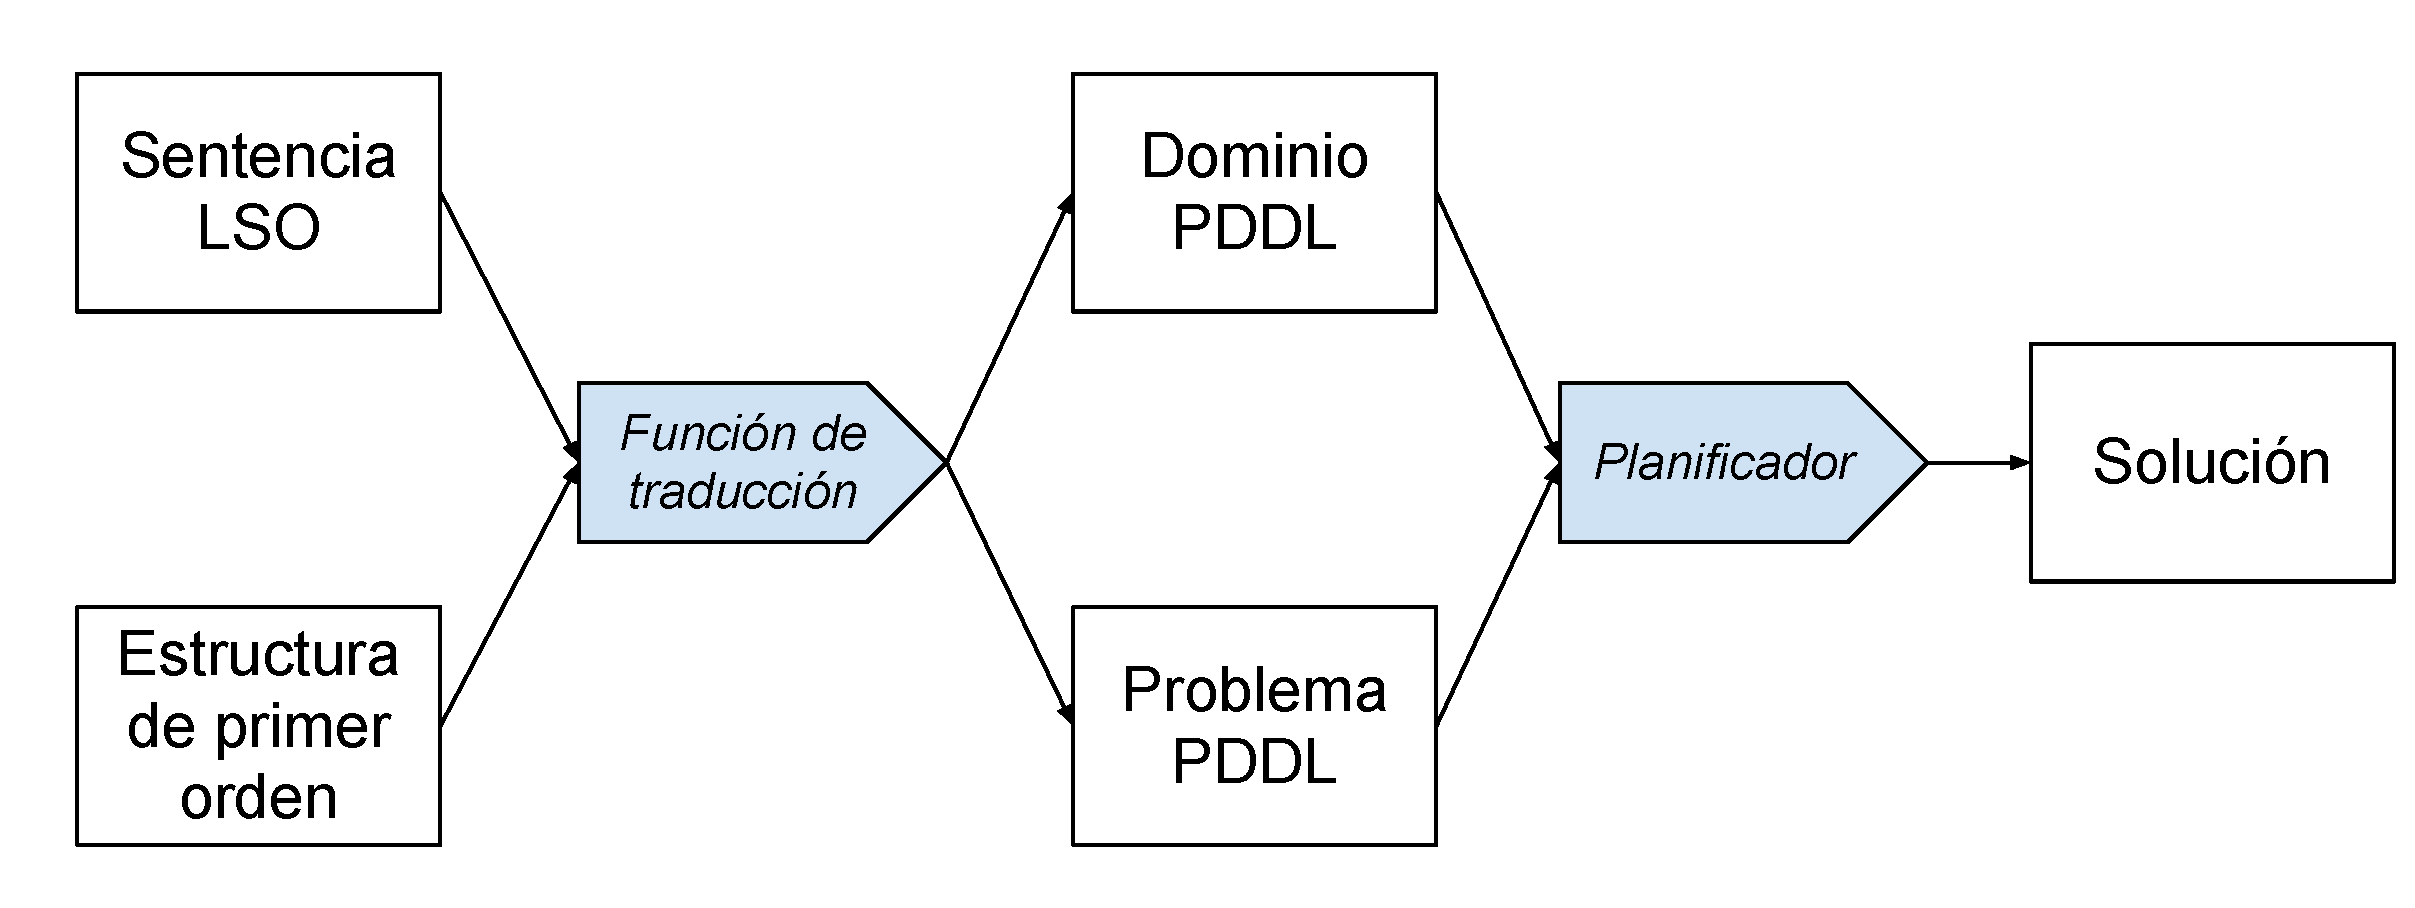
\includegraphics[width=\textwidth]{figuras/esquema_herramienta.pdf}
\caption[Grafo con una \textit{clique} de tamaño $k = 6$]{Grafo con una clique de tamaño
$k = 6$}
\label{clique}
\end{figure}

\begin{verbatim}
(exists F in Inj)(forall x y)[f(x) < K & f(y) < K -> E(x,y)]
\end{verbatim}

\subsection{\CHD, Camino Hamiltoniano Dirigido}
Esta fórmula expresa que existe una manera ordenada $F(a,b)$ de visitar los nodos de grafo (la posición $a$ la tiene el nodo $b$), en
la que para toda posición $x$, si no es la última, entonces existe un nodo $y1$ que le corresponde esta posición, y además
a la siguiente posición $x2$ le corresponde otro nodo $y2$, y hay un arco entre $y1$ y $y2$.
\begin{verbatim}
(so-exists (?F Inj)
  (forall (?x)
    (implies (< ?x MAX)
             (exists (?y1)
               (and (?F ?x ?y1)
                 (exists (?y2)
                   (and
                     (exists (?x2) 
                       (and (SUC ?x ?x2) (?f ?x2 ?y2)))
                   (?E ?y1 ?y2))))))))
\end{verbatim}
\begin{verbatim}
; (exists F in Inj)(forall x)[x < MAX -> E(f(x),f(x+1))]
\end{verbatim}

\subsection{\TDM, \textit{3-Dimensional Matching}}
\begin{verbatim}
(so-exists (?F Inj)
  (so-exists (?G Inj)
    (and
      (forall (?x) (exists (?y) (?F ?x ?y))) ; F is total
      (forall (?x) (exists (?y) (?G ?x ?y))) ; G is total
      (forall (?x) (forall (?y) (forall (?z)
        (implies (and (?F ?x ?y) (?G ?x ?z))
                 (?T ?x ?y ?z))))))))
\end{verbatim}

\subsection{\TCOL, 3-colorabilidad}
Esta fórmula expresa que existe una asignación de colores $R$, $G$ y $B$ tal que para todos los nodos
de un grafo, no hay dos vertices adyacentes del mismo color, los vertices tienen
almenos y a lo sumo un color.
\begin{verbatim}
(so-exists (?R 1) (so-exists (?G 1) (so-exists (?B 1)
  (forall (?x) 
    (and
      ; no hay dos vértices adyacentes del mismo color
      (forall (?y)
        (implies (?E ?x ?y) (not (or (and (?R ?x) (?R ?y))
                                        (and (?G ?x) (?G ?y))
                                        (and (?B ?x) (?B ?y))))))

        ; los vértices tienen al menos un color
        (or (?R ?x) (?G ?x) (?B ?x))

        ; los vértices tienen a lo sumo un color
        (implies (?R ?x) (and (not (?G ?x)) (not (?B ?x))))
        (implies (?G ?x) (and (not (?R ?x)) (not (?B ?x))))
        (implies (?B ?x) (and (not (?R ?x)) (not (?G ?x)))))))))
\end{verbatim}

\subsection{\KCOL, k-colorabilidad}
Esta fórmula expresa que existe una función de asignación de colores $F$, tal que a todo nodo se le es
asignado un color $y$, donde $K(y)$ quiere decir que el color $y$ es menor al máximo color
$k$; ademá, para todos los otros nodos, si este esta conectado a ellos, no
tienen el mismo color.

\begin{verbatim}
(so-exists (?F Func)
  (forall (?x) 
    (and (exists (?y) (and (?F ?x ?y) (?K ?y)))
      (forall (?y) 
        (implies (?E ?x ?y)
                 (not (exists (?z)
                   (and (?F ?x ?z) (?F ?y ?z)))))))))
\end{verbatim}

\section{Problemas PH}

\subsection{UNSAT, No-Satisfacibilidad proposicional}
Esta fórmula expresa que para toda relación $T$ sobre variables
proposicionales, existe una cláusula $y$ tal que para cada variable $x$, o $x$
aparece positiva en $y$ y $x$ es falsa, o $x$ aparece negativa en $y$ y $x$ es
verdadera, o $x$ no aparece en $y$.
\begin{verbatim}
(so-forall (?T 1 @ist)
    (exists (?y @cls)
        (forall (?x @var)
            (or (and (?N ?x ?y)
                     (?T ?x)
                )
                (and (?P ?x ?y)
                    (not (?T ?x))
                )
                (?NotIn ?x ?y)
             ))))
\end{verbatim}

\subsection{\qEA-QBF, Fórmula \textit{booleana} cuantificada $\Sigma_p^2$}
Esta fórmula expresa que existe una relación $E0$ sobre variables
proposicionales, tal que para toda relación $A0$ sobre variables
proposicionales, Para toda cláusula $c$ existe una variable $x$, tal que: o $x$ aparece
positiva en $c$ y es verdadera existencial o universalmente, o $x$ aparece negativa en $c$ y
es negativa existencial o universalmente.
\begin{verbatim}
(so-exists (?E0 1 @ise0)
    (so-forall (?A0 1 @isa0)
        (forall (?c @cls)
            (exists (?x @var)
                (or
                    (and (?P ?x ?c) (?E0 ?x))
                    (and (?P ?x ?c) (?A0 ?x))
                    (and (?N ?x ?c) (not (?E0 ?x)))
                    (and (?N ?x ?c) (not (?A0 ?x)))
                )))))
\end{verbatim}

\subsection{\coCOL, No-3-Colorabilidad}
Esta fórmula expresa que para toda posible coloración de nodos $R$, $G$ y $not-G \land not-R$, o dos nodos unidos por un arco tienen
el mismo color, o un nodo tiene dos colores al mismo tiempo.
\begin{verbatim}
(so-forall (?R 1 @node)
    (so-forall (?G 1 @node)
        (exists (?x @node)
            (or 
                (exists (?y @node)
                    ; no two adjacent vertices of the same color
                    (or (and (?E ?x ?y) (?R ?x) (?R ?y))
                        (and (?E ?x ?y) (?G ?x) (?G ?y))
                        (and (?E ?x ?y) (not (?R ?x)) 
                             (not (?R ?y)) (not (?G ?x)) 
                             (not (?G ?y)))
                    )
                )
                (and (?R ?x) (?G ?x))))))
\end{verbatim}


\addtocontents{toc}{\vspace{2em}}  % Add a gap in the Contents, for aesthetics
\backmatter

%% ----------------------------------------------------------------
\label{Bibliography}
\lhead{\emph{Bibliografía}}  % Change the left side page header to "Bibliography"
\bibliographystyle{alpha}  % Use the "unsrtnat" BibTeX style
%the Bibliography 
\bibliography{bibliografia}  % The references (bibliography) information are stored in the file named "Bibliography.bib"

\end{document}
